\documentclass[11pt,a4paper]{article}

\usepackage[T1]{fontenc}
\usepackage[utf8]{inputenc}
\IfFileExists{lmodern.sty}{\usepackage{lmodern}}{}
\usepackage[margin=2.6cm]{geometry}
\usepackage{amsmath,amssymb,amsthm}
\usepackage{mathtools}
\usepackage{booktabs}
\usepackage{tabularx}
\usepackage{multirow}
\usepackage{graphicx}
\usepackage[table]{xcolor}
\usepackage{tikz}
\usetikzlibrary{positioning,arrows.meta,shapes.geometric,calc,fit}
\usepackage{algorithm}
\usepackage{algpseudocode}
\usepackage{enumitem}
\usepackage{caption}
\usepackage{placeins}
\usepackage[round,authoryear]{natbib}
\usepackage[colorlinks=true,linkcolor=blue!50!black,citecolor=blue!50!black,urlcolor=blue!50!black]{hyperref}
\usepackage[capitalise,noabbrev]{cleveref}
\makeatletter
\providecommand*{\theHALG@line}{\thealgorithm.\arabic{ALG@line}}
\makeatother

\captionsetup{font=small,labelfont=bf}
\setlist{itemsep=2pt,topsep=4pt}
\setlength{\emergencystretch}{2em}

% ---------------------------------------------------------------- theorems
\newtheorem{proposition}{Proposition}
\newtheorem{corollary}{Corollary}
\theoremstyle{definition}
\newtheorem{definition}{Definition}
\newtheorem{remark}{Remark}

% ---------------------------------------------------------------- macros
% (the first block is shared with the symbolic-regression manuscript)
\newcommand{\R}{\mathbb{R}}
\newcommand{\E}{\mathbb{E}}
\newcommand{\D}{\mathcal{D}}
\newcommand{\bth}{\boldsymbol\theta}
\newcommand{\hth}{\hat\bth}
\newcommand{\bdelta}{\boldsymbol{\delta}}
\newcommand{\Fis}{\mathcal{I}}
\newcommand{\Fhat}{\widehat{\Fis}}
\newcommand{\KL}{D_{\mathrm{KL}}}
\DeclareMathOperator*{\argmin}{arg\,min}
\DeclareMathOperator*{\argmax}{arg\,max}
\DeclareMathOperator{\sgn}{sgn}
\DeclareMathOperator{\rank}{rank}
\DeclareMathOperator{\range}{range}
% this document
\newcommand{\keff}{k_{\mathrm{eff}}}
\newcommand{\Dtr}{\D_{\mathrm{tr}}}
\newcommand{\Dsel}{\D_{\mathrm{sel}}}
\newcommand{\DA}{\D_{A}}
\newcommand{\DB}{\D_{B}}
\newcommand{\Dte}{\D_{\mathrm{te}}}
\newcommand{\Mv}{\mathcal{M}}
\newcommand{\dbar}{\bar{\Delta}}
\newcommand{\sehat}{\widehat{\mathrm{SE}}}
\newcommand{\code}[1]{\texttt{#1}}
\newcommand{\WS}{\textsf{W+S}}
\newcommand{\Wo}{\textsf{W}}
\newcommand{\So}{\textsf{S}}
\newcommand{\todo}[1]{{\color{red!70!black}\sffamily\small[TODO: #1]}}

\definecolor{accent}{HTML}{2A78D6}
\definecolor{muted}{HTML}{8F8D86}

\title{Boundary pruning for neural networks:\\[2pt]
\large geometry proposes, held-out data decides\\[2pt]
\normalsize\textit{Working draft --- method and preliminary results}}
\author{Veronica Guidetti}
\date{\today}

\begin{document}
\maketitle

\begin{abstract}
We transfer a post hoc reduction framework developed for fitted symbolic-regression
models to neural networks. A pruning move takes the network to a boundary of its
compactified parameter space: a weight to zero, a unit to the constant it saturates
to or to its mean, a first-layer unit to a Heaviside step, a pair of near-duplicate
units to one unit, an attention head to a uniform or input-independent pattern, a
query--key or value--output product to lower rank. Every limit is realised exactly,
by a folded constant, a step unit, a fixed pattern or a factor of a weighted singular
value decomposition, and never by a large number. The move catalogue therefore follows
from the architecture. Identifiability decides which kind of decision a move needs.
Directions that are exactly null, detected with a gap test on block Fisher spectra,
can be quotiented out without any statistic. Sloppy directions have no valid local
Fisher statistic and are left to held-out data. Every move type then goes through one
rule: an anchored paired test against the original network, a paired tie set, and
a tie-break on the number of remaining parameters. No retraining is used anywhere.
On two toy models, a sigmoid MLP on two moons and a one-layer transformer trained
from scratch on $a+b \bmod 59$, the composite (structural) moves remove 94--97\% of
the MLP parameters at unchanged test accuracy. Single-parameter moves under the same rule
remove 10--21\%, and the Fisher-distance schemes of \citet{berman2026fdist} remove
6--9\%. At 70\% of the parameters removed the transformer keeps test accuracy 1.00,
against at most 0.12 for the Fisher-distance schemes. A crossed design
shows that the advantage comes from the composite moves and not from using held-out
data to choose them. On the transformer the gap test recovers, exactly, the
query--key null dimension predicted from the input geometry (1988 of 2048 per head).
These results are preliminary, and \cref{sec:outlook} lists what is needed before
they can be called credible.
\end{abstract}

\tableofcontents

% =============================================================================
\section{Introduction}
\label{sec:intro}

Pruning a trained neural network means choosing a smaller network inside, or at the
edge of, the parametric family of the original one, while preserving its predictive
behaviour. The dominant approaches score single coordinates: the magnitude
$|\theta_j|$ \citep{han2015learning}, a second-order estimate of the loss increase
\citep{lecun1990obd,hassibi1993obs,singh2020woodfisher}, a first-order Taylor term
\citep{molchanov2017taylor}, or an activation-weighted magnitude
\citep{sun2024wanda}. A growing family uses the Fisher information for the same
purpose \citep{theis2018fisher,liu2021groupfisher,kwon2022fast}. The most recent
member scores each coordinate by the Fisher--Rao length of the straight path that
takes it to zero, $s_k=\sqrt{\Fis_{kk}}\,|\theta_k|$ \citep{berman2026fdist}. It
descends from Bayesian renormalisation \citep{berman2023,howard2025} and from
sloppy-model reduction \citep{transtrum2011geometry,machta2013,transtrum2014}.

Our starting point is a framework for reducing \emph{fitted symbolic-regression (SR)
models} \citep{guidetti2026emergent}. That framework alternates three steps.
\emph{Propose}: local Fisher geometry nominates a few interpretable constraints.
\emph{Realise}: each constraint is applied exactly to the expression, which is then
contracted. \emph{Decide}: a predictive gate under cross-validation accepts at most
one move, and a parsimony criterion breaks ties. Two observations from that work
motivate this one.
\begin{enumerate}[label=(\roman*)]
\item Removable structure is not only small coefficients. Limits at infinity
(saturating subexpressions), signed identifications of parameters, and constant
subtrees remove whole subtrees. A zero-only rule leaves these in place or replaces
them by spurious constants.
\item Fisher-based statistics are only meaningful at identifiable points. Unidentifiable
directions make the Fisher matrix singular and corrupt every Wald-type statistic
computed on the same model, so they must be detected and removed first and separately.
\end{enumerate}

Both observations are sharper for neural networks than for symbolic expressions.
Neural networks are singular models in the sense of \citet{watanabe2009algebraic}.
Permutations of hidden units, sign and scale symmetries, duplicate units and dead
units make the map from parameters to functions many-to-one and the Fisher matrix
degenerate
\citep{sussmann1992uniqueness,fukumizu1996regularity,fukumizu2000local,amari2006singularities,wei2023singular}.
Attention adds a continuous $GL(d_h)$ gauge to every query--key and value--output
product \citep{elhage2021framework}. Saturating nonlinearities (sigmoid, softmax) put
boundaries of the function space at infinite parameter values. A coordinate score
such as $s_k$ is therefore the length of one path to one boundary, not the distance
to the pruned submodel (\cref{prop:singular}).

Three differences with the SR setting shape the transfer.
\begin{itemize}
\item \emph{No refitting.} In SR every candidate is refitted. A network is not
retrained after a move here, so whatever compensation a move needs has to be part of
the move, in closed form. For example, a unit replaced by a constant has that constant
folded into the next bias.
\item \emph{Held-out data are plentiful.} The $K$-fold cross-validation gate of the SR
operator becomes a paired test on a held-out split. The paired test is more powerful
for the same data, because all candidates are evaluated on the same samples.
\item \emph{The setting is $M$-open} \citep{bernardo1994bayesian}. Regular asymptotics
fail at the boundaries the method visits
\citep{chernoff1954distribution,self1987asymptotic,watanabe2009algebraic}, and the
family is never assumed to contain the truth. So we drop the BIC tie-break of the SR
operator \citep{schwarz1978estimating,grunwald2017inconsistency}. Among candidates
that the data cannot separate, we prefer the one with the fewest remaining parameters.
\end{itemize}

\paragraph{The idea in three principles.}
\begin{enumerate}[label=\textbf{P\arabic*.}]
\item \textbf{Every move is a limit of the parametrisation, realised exactly.} The
moves are not a hand-picked list of heuristics. Each is the limit of the network along
a path to a boundary stratum of the compactified parameter space, or along a null
direction. So the move set follows from the architecture: ask what each block becomes
at its limits. Limits are stored by their exact representative (a folded constant, a
step unit, a fixed attention pattern, a factorisation), never by a large number.
\item \textbf{Identifiability decides which kind of decision a move needs.} An exact
redundancy (a structural null of the Fisher matrix) can be removed at zero predictive
cost. Its removal is checked numerically, not tested statistically. A sloppy
redundancy has no valid local statistic and is decided by held-out data. Fisher
geometry is used only where it means something: to propose candidates and to detect
exact nulls. It never decides a sloppy move.
\item \textbf{One decision rule for all move types.} Each move is chosen by a paired
test anchored at the original network. Candidates the data cannot separate form a tie
set, and the tie is broken by the number of remaining parameters, so weight, unit,
head and rank moves compete on equal terms.
\end{enumerate}

\paragraph{What is classical and what is not.}
Most moves are known one by one. Removing a unit whose output is constant, folding it
into a bias, and merging units with duplicate or opposite outputs go back to
\citet{sietsma1988pruning}. Least-squares compensation of removed units is due to
\citet{castellano1997iterative}, and mean (``baseline'') compensation reappears in
FLAP \citep{an2024flap}. Neuron merging \citep{srinivas2015datafree,kim2020merging},
head pruning and mean ablation \citep{michel2019sixteen,voita2019heads,wang2023ioi},
and activation- or Fisher-weighted low-rank factorisation
\citep{hsu2022fwsvd,yuan2023asvd,wang2025svdllm} are established too. The idea of
reducing a model by moving to a boundary of its manifold and evaluating the limit
analytically is that of the manifold boundary approximation method
\citep{transtrum2014}. What we believe to be new is the combination:
\begin{itemize}
\item treating all of these moves as boundary limits of one compactified parameter
space, which adds saturation and Heaviside endpoints;
\item the split of redundancies into exact and sloppy by a gap test on network blocks,
with the consequence that the two are decided in different ways;
\item the argument that coordinate Fisher lengths are not distances in singular models;
\item one anchored selection rule over all move types, with complexity counted as live
parameters after structural cascades.
\end{itemize}

\paragraph{Status.} This is a proof of concept on two toy models
(\cref{sec:setup}). The headline results (\cref{sec:results}) are strong, but they rest
on one MLP task with three seeds and one transformer seed. The compensation built
into the structural moves has not been ablated, and the exact-quotient stage of the
method exists only as diagnostics. \Cref{sec:outlook} is a list of what remains to be
done before the claims are credible.

% =============================================================================
\section{Related work}
\label{sec:related}

\subsection{Parameter-level pruning}
\label{sec:rel-param}

Magnitude pruning zeroes the smallest weights and retrains \citep{han2015learning}.
Optimal Brain Damage (OBD) ranks weights by a diagonal second-order estimate of the
loss increase \citep{lecun1990obd}. Optimal Brain Surgeon (OBS) uses the full inverse
Hessian, and in doing so also updates the remaining weights to compensate
\citep{hassibi1993obs}. WoodFisher \citep{singh2020woodfisher} and SparseGPT
\citep{frantar2023sparsegpt} make OBS-type compensation scale. First-order
(Taylor) criteria \citep{molchanov2017taylor}, movement pruning
\citep{sanh2020movement} and Wanda's activation-weighted magnitude
\citep{sun2024wanda} are cheaper variants. Iterative magnitude pruning with rewinding
underlies the lottery-ticket line \citep{frankle2019lottery}.
\citet{hoefler2021sparsity} and \citet{blalock2020state} survey the area. The latter
also documents how hard fair comparisons are: different stopping rules, retraining
budgets and complexity counts.

All these methods move one coordinate at a time to zero. Compensation, where it
exists, is a least-squares update of the remaining weights. Our single-parameter
moves (\cref{sec:moves-weights}) are of this kind and serve as a control.

\subsection{Fisher geometry, sloppiness and Fisher-distance pruning}
\label{sec:rel-fisher}

The Fisher information is the natural metric on a statistical model
\citep{amari2000methods,amari2016}. Fisher-based pruning estimates the loss change of
removing a parameter or group from the empirical Fisher
\citep{theis2018fisher,liu2021groupfisher}. EigenDamage prunes in a Kronecker-factored
eigenbasis \citep{wang2019eigendamage}. \citet{kwon2022fast} search head and filter
masks of a trained Transformer under a Fisher-based constraint and then rescale the
remaining weights by layer-wise least squares, without retraining. Theirs is the
closest existing post-training structured pipeline.

In the physics literature, nonlinear models are ``sloppy'': their Fisher spectra span
many decades, and only a few stiff combinations are constrained by data
\citep{transtrum2011geometry,machta2013,transtrum2015,Quinn2021}. The manifold boundary
approximation method (MBAM) of \citet{transtrum2014} follows a geodesic along the
sloppiest direction until the model manifold reaches a boundary. There parameters go
to limiting values, typically $0$ or $\infty$, and a reduced model is read off
analytically. This is the precedent for our principle P1. Bayesian renormalisation
\citep{berman2023,howard2025} integrates out directions that cannot be resolved at a
given information scale. Its implementation for neural networks
\citep{berman2026fdist} ranks parameters by
\begin{equation}
s_k(\bth) = \sqrt{\Fis_{kk}(\bth)}\;|\theta_k|,
\label{eq:berman}
\end{equation}
the first-order Fisher--Rao length of the coordinate path $\theta_k\to0$. Its variants
evaluate the metric at the dense model (one-shot), at the running pruned model
(iterative), averaged along a global rescaling (global), or along the coordinate
path itself (exact). All of them are global, unstructured and zero-only. We use their
code as a baseline (\cref{sec:baselines}) and as the single-parameter proposer in our
controlled comparison.

\Cref{prop:singular} shows that \eqref{eq:berman} is an upper bound on the local
Fisher distance to the submodel $\{\theta_k=0\}$, with equality only when coordinate
$k$ is Fisher-orthogonal to all others. The bound is attained by $0$, not by $s_k$,
whenever $k$ takes part in a null direction. In a singular model this is the generic
case for redundant parameters.

\subsection{Structural moves}
\label{sec:rel-struct}

\paragraph{Units.} \citet{sietsma1988pruning,sietsma1991creating} removed hidden units
whose outputs are constant over the training set, adding the constant to the
downstream biases, and units whose outputs duplicate or mirror another unit's, folding
them into it. \citet{castellano1997iterative} showed that these rules are special
consistency conditions of a linear system that preserves every downstream net input,
which they solve in the least-squares sense. FLAP \citep{an2024flap} adds the removed
channels' mean contribution as a bias in large language models. Data-free merging of
similar neurons \citep{srinivas2015datafree} and merging with a learned scaling matrix
\citep{kim2020merging} complete this line. Our \code{unit\_mean} and \code{unit\_merge}
moves are these, written as boundary limits.

\paragraph{Heads.} Many attention heads can be removed at inference with little loss
\citep{michel2019sixteen,voita2019heads}. Replacing a component's output by its mean is
the standard ablation of mechanistic interpretability \citep{wang2023ioi}. Our
\code{head\_off} and \code{head\_mean} moves are these.

\paragraph{Low rank.} Low-rank factorisation of trained weights goes back at least to
\citet{denton2014linear}. Weighting the reconstruction by Fisher information
\citep{hsu2022fwsvd} or by input activations \citep{yuan2023asvd,wang2025svdllm}
makes the truncation aware of the data. SliceGPT \citep{ashkboos2024slicegpt} exploits
an exact orthogonal invariance of the residual stream to delete rows and columns.
Our \code{qk\_rank} and \code{ov\_rank} moves are activation-weighted truncations of
the $W_QW_K^\top$ and $W_VW_O$ products, one rank at a time.

\paragraph{What is missing.} We are not aware of pruning methods that treat sigmoid
saturation, the Heaviside limit of a unit, or the zero- and infinite-temperature limits
of softmax as moves. Nor are we aware of methods that put unit, head, rank and weight
moves under one statistical decision rule. Structured LLM pruners
\citep{ma2023llmpruner,an2024flap,ashkboos2024slicegpt} fix one granularity and one
importance score per method.

\subsection{Singular models, identifiability and model selection}
\label{sec:rel-singular}

\citet{sussmann1992uniqueness} showed that minimal $\tanh$ networks are identifiable
up to permutations and sign flips. Non-minimal networks (duplicate, constant or dead
units) are not. \citet{fukumizu1996regularity} characterised when the Fisher matrix of
a multilayer perceptron is singular. \citet{fukumizu2000local} and
\citet{amari2006singularities} showed that such singular regions shape the learning
dynamics. Singular learning theory \citep{watanabe2009algebraic,watanabe2013widely}
replaces the parameter count of regular asymptotics by the real log canonical
threshold. Its local estimate, the local learning coefficient \citep{lau2025llc}, is a
singularity-aware complexity measure for trained networks \citep{wei2023singular}.
Rescaling symmetries also make Hessian-based quantities coordinate-dependent
\citep{dinh2017sharp}. Fisher spectra of deep networks are dominated by near-zero
eigenvalues \citep{karakida2019universal}. Identifiability analysis distinguishes
structural from practical non-identifiability \citep{raue2009structural}. This is
exactly the distinction between the exact and sloppy nulls of principle P2.

Tests at boundaries of the parameter space have non-standard limits
\citep{chernoff1954distribution,self1987asymptotic}, and Wald statistics need an
interior, identifiable point \citep{wald1943tests}. Our tie rule is a paired version
of the one-standard-error rule \citep{breiman1984classification,hastie2009elements}.
Reusing one validation split to choose many moves overfits it
\citep{cawley2010overfitting,dwork2015reusable}. This motivates the separation of
selection and stopping data in \cref{sec:decide}.

\begin{table}[t]
\centering\footnotesize
\caption{Positioning relative to the families of methods discussed above. ``Comp.''
is the compensation applied to the surviving parameters when something is removed.}
\label{tab:related}
\renewcommand{\arraystretch}{1.25}
\begin{tabularx}{\textwidth}{@{}p{2.7cm}XXp{2.3cm}X@{}}
\toprule
\textbf{Family} & \textbf{Target} & \textbf{Admissible reductions} & \textbf{Comp.} & \textbf{Decision rule}\\
\midrule
Magnitude, OBD, Taylor, Wanda & single weights & zero & none (retrain) & score threshold at a fixed sparsity\\
OBS, WoodFisher, SparseGPT & single weights & zero & least-squares update & score threshold at a fixed sparsity\\
Fisher distance \citep{berman2026fdist} & single weights & zero & none & score threshold at a fixed sparsity\\
Unit removal / merging & hidden units & constant, duplicate & bias fold, merge & heuristic thresholds\\
Head pruning, mean ablation & heads & zero, mean & bias (mean) & importance score\\
Low-rank (FWSVD, ASVD, SVD-LLM) & weight matrices & rank truncation & weighted SVD & target rank or ratio\\
\citet{kwon2022fast} & heads, filters & zero & layer-wise least squares & Fisher-constrained mask search\\
MBAM & sloppy combinations & manifold boundaries ($0$, $\infty$) & refit & boundary reached along a geodesic\\
\midrule
\textbf{This work} & \textbf{weights, units, heads, products} & \textbf{zero, constant, saturation ($\pm\infty$), step, duplicate, rank, uniform / fixed attention} & \textbf{exact folds, merges, weighted SVD} & \textbf{anchored paired test on held-out data, paired tie set, fewest parameters}\\
\bottomrule
\end{tabularx}
\end{table}

% =============================================================================
\section{Preliminaries}
\label{sec:prelim}

\subsection{Setting and notation}
\label{sec:setting}

A trained network $f(\cdot\,;\bth,\sigma)$ maps an input $x$ to logits $z\in\R^{C}$
($C=1$ for a Bernoulli output). Its predictive distribution is
$p(y\mid x;\bth,\sigma)=\mathrm{softmax}(z)_y$, or $\mathrm{sigmoid}(z)$ in the
Bernoulli case. Here $\bth\in\R^{p}$ collects the continuous parameters and $\sigma$
is a discrete \emph{structural state}. The structural state records which units are
active, removed or replaced by a step, which heads are alive or have a fixed
attention pattern, and which entries of $\bth$ are masked. Moves change both. The
per-sample criterion is either the log loss $\ell(x,y;f)=-\log p(y\mid x;f)$ or the
$0/1$ error $e(x,y;f)$; we write $c$ for whichever is in use. The data are split into
a training set $\Dtr$, a validation set, and a test set $\Dte$. In the controlled
design of \cref{sec:fair}, the validation set is halved once, at random, into $\DA$
and $\DB$. The test set is never used for any decision.

The (expected, model) Fisher information at $\bth$ over an input population $P_X$ is
\begin{equation}
\Fis(\bth)=\E_{x\sim P_X}\,\E_{y\sim p(\cdot\mid x;\bth)}
\big[\nabla_{\bth}\log p(y\mid x;\bth)\,\nabla_{\bth}\log p(y\mid x;\bth)^{\!\top}\big]
=\E_{x\sim P_X}\big[J(x)^{\top}H(x)\,J(x)\big],
\label{eq:fisher}
\end{equation}
with $J=\partial z/\partial\bth$ and $H=\mathrm{diag}(\pi)-\pi\pi^{\top}$, where
$\pi=\mathrm{softmax}(z)$; in the Bernoulli case $H=\pi(1-\pi)$. For these likelihoods
$\Fis$ coincides with the generalised Gauss--Newton matrix of the log loss. In the
Bernoulli case we compute it exactly. In the categorical case we estimate it by Monte
Carlo, with $R$ labels drawn from the model per input. Every Monte Carlo score vector
lies in the row space of $J(x)$, so structural null directions stay exactly null
and the sampling only adds noise to the retained part. We use two versions. The
\emph{diagonal} $\Fhat_{jj}$, summed over $\Dtr$, serves for proposals
(\cref{sec:moves-weights}). The \emph{block} matrix $\Fis_B$ of a group of parameters
$B$ (a head's query--key pair, a unit's fan-in and fan-out, or a whole small
network), summed over all available inputs, serves for the identifiability test
(\cref{sec:stage1}).

\subsection{Moves as boundary limits}
\label{sec:moves-def}

\begin{definition}[Move]
\label{def:move}
A \emph{move} $m$ at the current network $f=f(\cdot\,;\bth,\sigma)$ consists of a path
$t\mapsto\gamma_m(t)\in\R^{p}$, $t\in[0,t^\ast)$, with $\gamma_m(0)=\bth$, together with
a \emph{representative} $(\bth_m,\sigma_m)$, such that the networks
$f(\cdot\,;\gamma_m(t),\sigma)$ converge pointwise on the input domain, as $t\to t^\ast$,
to a network $f_m=f(\cdot\,;\bth_m,\sigma_m)$ with fewer live parameters. The path may
reach a finite point (a weight to zero), go to infinity (a bias to $-\infty$), or run
along a null direction of $\Fis$ (two duplicate units collapsing into one).
\end{definition}

The representative is what is stored. A limit is never approximated by a large number:
a saturated unit is deleted and its constant output added to the next bias, a unit in
its Heaviside limit is stored as the pair (input index, sign), and a head at the
input-independent limit of its softmax is stored as a fixed pattern. Whatever
compensation the remaining network needs is therefore part of the limit and is exact,
not fitted. When the limit leaves a free constant (the value of a constant unit), we
pick the point of the boundary stratum closest to the current network in the $L^2$
sense of its activations, which is the training mean.

\begin{definition}[Live parameters $\keff$]
\label{def:keff}
After every move the network is \emph{canonicalised}: the following rules are applied
until nothing changes.
\begin{enumerate}[label=(\roman*)]
\item A unit without live outgoing weights is removed together with its fan-in and bias.
\item A unit without live incoming weights is a constant ($\mathrm{sigmoid}(b_i)$ or
$\mathrm{ReLU}(b_i)$), which is folded into the next bias and then removed.
\item In an attention head, a head-dimension column of $W_Q$ ($W_V$) is removed when the
matching column of $W_K$ (row of $W_O$) is dead, and vice versa.
\item A head without live value--output columns is removed.
\item A head with a fixed pattern loses its query--key weights.
\end{enumerate}
$\keff(f)$ is the number of live entries of all parameter tensors after
canonicalisation, plus the numbers a representative needs. A fixed causal pattern over
$T$ positions costs $T(T-1)/2$.
\end{definition}

Canonicalisation is itself an exact quotient. It removes the null directions that
earlier moves have \emph{induced}, without any statistic. Continuous gauge directions,
namely the positive rescaling of a ReLU unit and the $GL(d_h)$ freedom of the
$W_QW_K^{\top}$ and $W_VW_O$ factorisations, are not subtracted from $\keff$. They are
measured separately by the gap test of \cref{sec:stage1}.

\subsection{Fisher geometry at singular points}
\label{sec:singular}

Let $\Fis\succeq0$ be the Fisher matrix at $\bth$, and let
$\mathcal{M}_k=\{\bth':\theta'_k=0\}$ be the submodel in which coordinate $k$ is
pruned. Under the local quadratic approximation of the Kullback--Leibler divergence,
$\KL(\bth\,\|\,\bth+\bdelta)\approx\frac12\bdelta^{\top}\Fis\,\bdelta$, the squared
Fisher distance from $\bth$ to $\mathcal{M}_k$ is
\begin{equation}
d_k^{2}=\min_{\bdelta:\;\delta_k=-\theta_k}\;\bdelta^{\top}\Fis\,\bdelta .
\label{eq:dk}
\end{equation}
When $\Fis$ is invertible, $d_k^{2}=\theta_k^{2}/(\Fis^{-1})_{kk}$. This is the Wald
statistic for $\theta_k=0$ and the zero-boundary statistic of the SR operator
\citep{guidetti2026emergent}. It lets the other coordinates compensate, i.e.\ it is
\emph{profiled}. The score \eqref{eq:berman} moves $\theta_k$ alone:
$s_k^{2}=\theta_k^{2}\,\Fis_{kk}$.

\begin{proposition}[Coordinate length versus distance to the pruned submodel]
\label{prop:singular}
Let $\Fis\succeq0$ and let $\Fis^{+}$ be its Moore--Penrose inverse.
\begin{enumerate}[label=(\alph*)]
\item If $\ker\Fis$ contains a vector $v$ with $v_k\neq0$, then $d_k=0$.
\item Otherwise $e_k\in\range\Fis$ and $d_k^{2}=\theta_k^{2}/(\Fis^{+})_{kk}$.
\item In both cases $d_k\le s_k$. For $\theta_k\neq0$ equality holds if and only if
$\Fis_{kj}=0$ for every $j\neq k$.
\end{enumerate}
\end{proposition}

\begin{proof}
(a) $\bdelta=-(\theta_k/v_k)\,v$ satisfies the constraint and
$\bdelta^{\top}\Fis\bdelta=0$.
(b) Since $\Fis$ is symmetric, $\range\Fis=(\ker\Fis)^{\perp}$. If no kernel vector
has a non-zero $k$-th entry, then $e_k\perp\ker\Fis$ and $e_k\in\range\Fis$. Write
$\bdelta=\bdelta_R+\bdelta_N$ with $\bdelta_R\in\range\Fis$ and
$\bdelta_N\in\ker\Fis$. Then $(\bdelta_N)_k=0$, so the constraint reads
$e_k^{\top}\bdelta_R=-\theta_k$, and the objective is
$\bdelta_R^{\top}\Fis\bdelta_R$. On $\range\Fis$ the matrix $\Fis$ is positive definite with inverse $\Fis^{+}$, so
$(\Fis^{+})_{kk}=e_k^{\top}\Fis^{+}e_k>0$, and the problem is a strictly convex quadratic
under one linear constraint. Its unique minimiser, from the Lagrange condition, is
$\bdelta_R=-\theta_k\,\Fis^{+}e_k/(e_k^{\top}\Fis^{+}e_k)$, which uses
$\Fis\Fis^{+}e_k=e_k$, and the minimum is $\theta_k^{2}/(\Fis^{+})_{kk}$.
(c) In case (a) the claim is trivial. In case (b), let $P=\Fis\Fis^{+}$ be the
orthogonal projector onto $\range\Fis$. Then $Pe_k=e_k$ and, by Cauchy--Schwarz,
\[
1=e_k^{\top}Pe_k=\big\langle\Fis^{1/2}e_k,\,(\Fis^{+})^{1/2}e_k\big\rangle
\le\sqrt{\Fis_{kk}\,(\Fis^{+})_{kk}} .
\]
Hence $d_k^{2}=\theta_k^{2}/(\Fis^{+})_{kk}\le\theta_k^{2}\Fis_{kk}=s_k^{2}$.
Equality requires $\Fis^{1/2}e_k\parallel(\Fis^{+})^{1/2}e_k$. Multiplying by
$\Fis^{1/2}$ gives $\Fis e_k\parallel e_k$, i.e.\ $e_k$ is an eigenvector of $\Fis$,
which is the same as $\Fis_{kj}=0$ for all $j\neq k$. Conversely, let $e_k$ be an
eigenvector with eigenvalue $\lambda$. If $\lambda=0$, then $d_k=s_k=0$. If
$\lambda>0$, then $(\Fis^{+})_{kk}=1/\lambda=1/\Fis_{kk}$ and equality holds. In case (a)
with $\Fis_{kk}>0$, $e_k$ cannot be an eigenvector: it would lie in $\range\Fis$,
orthogonal to $v$. So there $d_k=0<s_k$.
\end{proof}

So $s_k$ is the length of one path, the coordinate path, to one point of
$\mathcal{M}_k$. The distance to the pruned model is never larger, and it is zero
whenever $\theta_k$ takes part in an exact redundancy. In a singular network this is
the typical situation for exactly the parameters one would like to prune.

\begin{corollary}[Duplicate units]
\label{cor:duplicate}
Suppose two hidden units have identical activations, $a_i(x)=a_{i'}(x)$ for $P_X$-almost
every $x$. For every downstream unit $u$, the direction that increases $W_{u i}$ and
decreases $W_{u i'}$ by the same amount leaves the function unchanged, so it lies in
$\ker\Fis$. Therefore the distance \eqref{eq:dk} to the submodel in which unit $i$'s
outgoing column is zero is $0$, however large $s_k$ is. The zero-distance path is the
merge of $i$ into $i'$, which is realised exactly by the \code{unit\_merge} move of
\cref{sec:moves-mlp} with $\alpha=1,\beta=0$.
\end{corollary}

On the moons MLP of \cref{sec:setup} (seed 123), two second-layer units have activation
correlation $0.99977$. The straight path that zeroes either unit's outgoing column has
Fisher length $\big(\sum_j\Fhat_{jj}w_j^2\big)^{1/2}\approx1.3$, with the diagonal Fisher
of the summed training loss. Zeroing one column increases the validation loss by
$+0.027$. Merging the two units changes it by $\pm4\times10^{-5}$.

\begin{remark}[Boundaries at infinity are reached along symmetry orbits]
\label{rem:infinity}
In $f(x)=a\,b\,x$ only $c=ab$ is identified. Along the orbit $ab=c\neq0$, the coordinate
boundary $a=0$ is reached only as $b\to\infty$. The same holds for the positive
rescaling of a ReLU unit, $(w_{\mathrm{in}},w_{\mathrm{out}})\mapsto
(\lambda w_{\mathrm{in}},w_{\mathrm{out}}/\lambda)$: shrinking the outgoing weights to
zero along the orbit sends the incoming weights to infinity. In a singular model, then,
zero boundaries and boundaries at infinity are two charts of the same compactified
orbit space. A pruning rule that only visits finite zeros sees half of it.
\end{remark}

\begin{remark}[No Fisher statistic decides a move]
\label{rem:calibration}
Wald-type calibration needs an interior, identifiable point and a smooth boundary
\citep{wald1943tests,chernoff1954distribution,self1987asymptotic}. At an exact null the
statistic is zero or undefined (\cref{prop:singular}). At a sloppy direction near a
boundary, including boundaries at infinity, its $\chi^{2}_{1}$ reading fails. The SR
operator already used Fisher statistics only as permissive screens
\citep{guidetti2026emergent}. Here we go one step further. Geometry only \emph{ranks}
candidates (\cref{sec:propose}) and \emph{detects} exact nulls (\cref{sec:stage1}).
Every decision that changes the function is taken on held-out data (\cref{sec:decide}).
\end{remark}

% =============================================================================
\section{Method}
\label{sec:method}

\subsection{Overview}
\label{sec:overview}

The procedure has two stages (\cref{fig:method}). \emph{Stage 1} quotients out the
exact nulls detected by a gap test on block Fisher spectra. The function does not
change, so no statistic is involved. \emph{Stage 2} is a greedy loop over moves that do
change the function. Geometry proposes candidates, each candidate is realised exactly
and canonicalised, a selection split chooses one move, and a separate stop split ends
the path. In the current implementation Stage 1 exists only as a diagnostic; exact
nulls are removed by ordinary moves inside Stage 2 (\cref{sec:stage1}).

\begin{figure}[t]
\centering
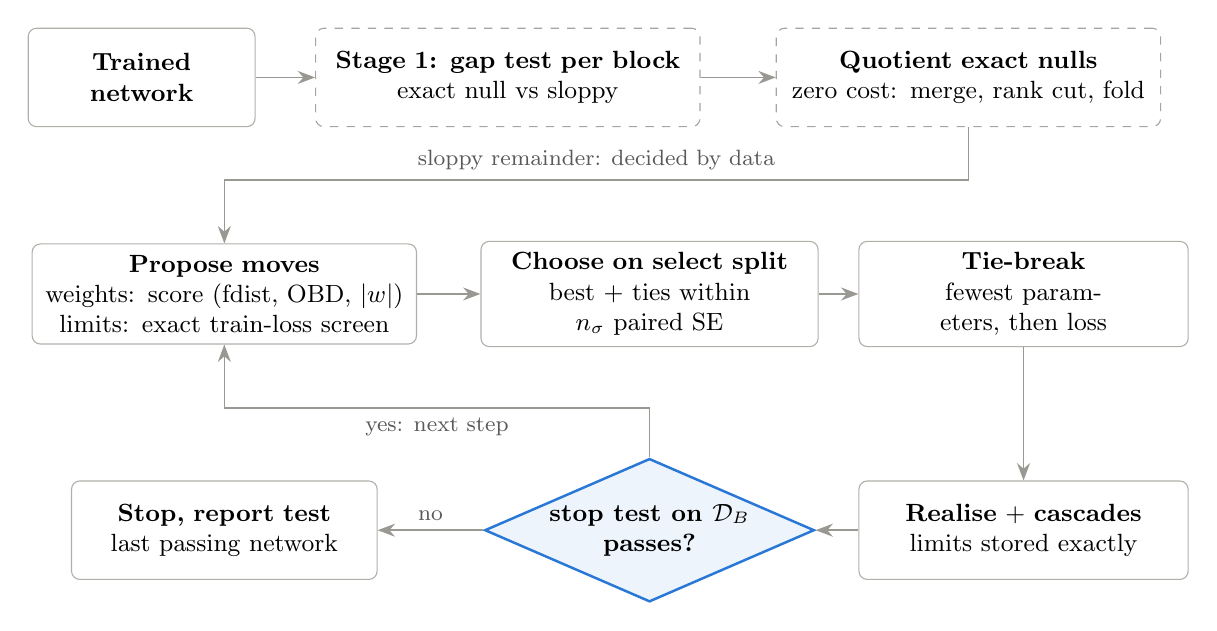
\begin{tikzpicture}[
  font=\small, >={Stealth[length=2.2mm]},
  box/.style={draw=muted!70, rounded corners=3pt, align=center, inner sep=4pt,
              minimum height=1.25cm, text width=#1},
  box/.default=3.6cm,
  plan/.style={box=#1, dashed, draw=muted!80},
  plan/.default=3.6cm,
  arr/.style={->, draw=muted!90, line width=0.6pt},
  lab/.style={font=\footnotesize, text=black!65}]
% row 1
\node[box=2.6cm] (net) at (0.5,0) {\textbf{Trained network}};
\node[plan=4.6cm] (gap) at (5.15,0) {\textbf{Stage 1: gap test per block}\\ exact null vs sloppy};
\node[plan=4.6cm] (quo) at (11.0,0) {\textbf{Quotient exact nulls}\\ zero cost: merge, rank cut, fold};
% row 2
\node[box=4.6cm] (prop) at (1.55,-2.75) {\textbf{Propose moves}\\ weights: score (fdist, OBD, $|w|$)\\ limits: exact train-loss screen};
\node[box=4.0cm] (sel) at (6.95,-2.75) {\textbf{Choose on select split}\\ best $+$ ties within $n_\sigma$ paired SE};
\node[box=3.9cm] (tie) at (11.7,-2.75) {\textbf{Tie-break}\\ fewest parameters, then loss};
% row 3
\node[box=3.9cm] (app) at (11.7,-5.75) {\textbf{Realise $+$ cascades}\\ limits stored exactly};
\node[diamond, aspect=2.3, draw=accent, line width=0.9pt, fill=accent!8, align=center,
      inner sep=0.5pt] (stop) at (6.95,-5.75) {\textbf{stop test on $\DB$}\\ \textbf{passes?}};
\node[box=3.6cm] (end) at (1.55,-5.75) {\textbf{Stop, report test}\\ last passing network};
% arrows
\draw[arr] (net) -- (gap);
\draw[arr] (gap) -- (quo);
\draw[arr] (quo.south) -- (quo.south |- 0,-1.3) -- node[lab, above, pos=0.5] {sloppy remainder: decided by data} (prop.north |- 0,-1.3) -- (prop.north);
\draw[arr] (prop) -- (sel);
\draw[arr] (sel) -- (tie);
\draw[arr] (tie) -- (app);
\draw[arr] (app) -- (stop);
\draw[arr] (stop) -- node[lab, above] {no} (end);
\draw[arr] (stop.north) -- (stop.north |- 0,-4.2) -- node[lab, below, pos=0.5] {yes: next step} (prop.south |- 0,-4.2) -- (prop.south);
\end{tikzpicture}
\caption{Geometry proposes, held-out data decides, and one stop rule ends every path.
Dashed boxes are planned as a separate stage. Today exact nulls are removed by ordinary
moves inside the loop. The select split is $\Dtr$ or $\DA$; the stop split $\DB$ is
used by every method, greedy or one-shot, and by nothing else.}
\label{fig:method}
\end{figure}

\subsection{Moves for a sigmoid MLP}
\label{sec:moves-mlp}

Write $a^{(0)}=x$ and $a^{(\ell)}_i=\mathrm{sigmoid}\big(w^{(\ell)\top}_{i}a^{(\ell-1)}
+b^{(\ell)}_i\big)$ for the hidden layers $\ell=1,\dots,L-1$. The output logit is
$z=W^{(L)}a^{(L-1)}+b^{(L)}$. A unit $i$ of layer $\ell$ has fan-in $d_{\ell-1}$, one
bias and fan-out $d_{\ell+1}$, where $W^{(\ell+1)}_{:,i}$ is its outgoing column. The
inputs are standardised, so their coordinates change sign. Deeper layers receive
sigmoid outputs, which are strictly positive. We write $\mathrm{fold}_i(c)$ for the
operation $b^{(\ell+1)}\leftarrow b^{(\ell+1)}+c\,W^{(\ell+1)}_{:,i}$ followed by
deletion of unit $i$ (its fan-in, bias and outgoing column).

\begin{description}[style=nextline, leftmargin=0.6cm, font=\normalfont\ttfamily]
\item[unit\_sat($c$), $c\in\{0,1\}$] Path $b_i\to-\infty$ ($c=0$) or $b_i\to+\infty$
($c=1$). Then $a_i\to c$ uniformly on bounded inputs. Representative:
$\mathrm{fold}_i(c)$. It frees $d_{\ell-1}+1+d_{\ell+1}$ parameters. For $\ell\ge2$ the
inputs of the unit lie in a compact subset of $(0,1)^{d_{\ell-1}}$, so the same
endpoint is reached by \emph{any single} incoming weight
$w_{ij}\to\pm\infty$. (This fails for an input that has been replaced by a Heaviside
step, whose output can be $0$.) The endpoint is a property of the unit even when the path moves
one weight.
\item[unit\_mean] Path $w^{(\ell)}_i\to0$ with $b_i$ set to
$\operatorname{logit}\bar a_i$, where $\bar a_i$ is the mean training activation. The
limit is the constant unit $a_i\equiv\bar a_i$, the $L^2$ projection of $a_i$ onto
constants. Representative: $\mathrm{fold}_i(\bar a_i)$. It frees the same parameters as
\code{unit\_sat}.
\item[unit\_step($j,s$)] Layer $\ell=1$ only. Path $w_{ij}\to s\cdot\infty$ with the
rest of the fan-in fixed. Then $a_i(x)\to H(s\,x_j)$ for $x_j\neq0$, where $H$ is the
Heaviside step. Representative: the pair $(j,s)$; the fan-in and the bias of the unit
are deleted and the outgoing column is kept. It frees $d_0+1$ parameters. In deeper
layers a single weight going to infinity gives a constant, not a step, because the
inputs are positive.
\item[unit\_merge($i\to i'$)] Fit $a_i\approx\alpha a_{i'}+\beta$ by least squares on
the training activations. Representative:
$W^{(\ell+1)}_{:,i'}\leftarrow W^{(\ell+1)}_{:,i'}+\alpha W^{(\ell+1)}_{:,i}$,
$b^{(\ell+1)}\leftarrow b^{(\ell+1)}+\beta W^{(\ell+1)}_{:,i}$, delete unit $i$. When
$a_i=\alpha a_{i'}+\beta$ holds exactly, the move runs along a null direction and does
not change the function (\cref{cor:duplicate}). With $\alpha=\pm1,\beta\in\{0,1\}$ it
is the duplicate / opposite-unit rule of \citet{sietsma1988pruning}. Candidates are
the $n_{\mathrm{merge}}$ pairs per layer with the largest $|\mathrm{corr}(a_i,a_{i'})|$,
in both directions.
\item[zero] A weight, or a chunk of weights, to $0$ (\cref{sec:moves-weights}).
\end{description}

\subsection{Moves for a one-layer transformer}
\label{sec:moves-tf}

The transformer reads a sequence of $T$ tokens. Its residual stream is
$x^{(0)}_t=E[\mathrm{tok}_t]+P_t$. A head $h$ computes
$q_t=x^{(0)\top}_tW^h_Q$, $k_t=x^{(0)\top}_tW^h_K$ and $v_t=x^{(0)\top}_tW^h_V$, with
$W^h_{Q},W^h_K,W^h_V\in\R^{d\times d_h}$. Its attention pattern is
$A^h_{ts}=\mathrm{softmax}_s\big(q_t^{\top}k_s/\sqrt{d_h}\big)$ over $s\le t$, and its
output is $o^h_t=\sum_sA^h_{ts}v_s^{\top}W^h_O$, with $W^h_O\in\R^{d_h\times d}$. Then
\begin{gather*}
x^{(1)}=x^{(0)}+\sum_ho^h+B_{\mathrm{attn}},\qquad
x^{(2)}=x^{(1)}+W_{\mathrm{out}}\,\mathrm{ReLU}\big(W_{\mathrm{in}}x^{(1)}+b_{\mathrm{in}}\big)+b_{\mathrm{out}},\\
z=W_U^{\top}x^{(2)}_T+b_U .
\end{gather*}
$B_{\mathrm{attn}}\in\R^{T\times d}$ is a per-position bias. It starts at zero, is not
trained, and becomes live only when a head is mean-ablated. There is no LayerNorm (so
no LayerNorm gauge) and there are no attention biases (so no key-bias null). Only the
last position $T$ reaches the loss. The activation statistics used below are therefore
taken there: $C_q=\E[x^{(0)}_Tx^{(0)\top}_T]$,
$C_k=\E[x^{(0)}_sx^{(0)\top}_s]$ over all positions $s$, and
$C^h_y=\E[y^hy^{h\top}]$ with $y^h=\sum_sA^h_{Ts}x^{(0)}_s$.

\begin{description}[style=nextline, leftmargin=0.6cm, font=\normalfont\ttfamily]
\item[head\_off] $o^h\to0$, e.g.\ $W_O^h\to0$. It frees $4dd_h$ parameters.
\item[head\_mean] $o^h_t\to\E[o^h_t]$, the training mean per position, added to
$B_{\mathrm{attn}}$. It frees $4dd_h$ and makes $B_{\mathrm{attn}}$ live ($Td$
numbers, counted once).
\item[attn\_uniform] The softmax temperature limit $s\to0$ in
$\mathrm{softmax}(s\,q^{\top}k)$, i.e.\ $W^h_QW^{h\top}_K\to0$. The pattern becomes
uniform over $s\le t$. Representative: $W^h_Q,W^h_K$ masked. It frees $2dd_h$.
\item[attn\_fixed] The pattern becomes constant in the input,
$A^h\equiv\bar A^h=\E[A^h]$. This stratum contains the hard-max limit $s\to\infty$
whenever the argmax does not depend on the input. Representative: the fixed causal
pattern. It frees $2dd_h$ and costs $T(T-1)/2$.
\item[qk\_rank] The rank of $M=W^h_QW^{h\top}_K$ is reduced from $r$ to $r-1$ by
\begin{equation}
M'=\argmin_{\rank M'\le r-1}\big\|C_q^{1/2}(M-M')C_k^{1/2}\big\|_F .
\label{eq:wsvd}
\end{equation}
If the query and key inputs were independent, the objective would be the expected
squared change of the attention logit, $\E[(x_q^{\top}(M-M')x_k)^2]$
(\cref{app:wsvd}). The minimiser is closed-form. Take the SVD
$C_q^{1/2}MC_k^{1/2}=U\Sigma V^{\top}$; then
$W_Q'=C_q^{-1/2}U_{r-1}\Sigma_{r-1}^{1/2}$ and
$W_K'=C_k^{-1/2}V_{r-1}\Sigma_{r-1}^{1/2}$. The eigenvalues of $C_q,C_k$ are floored at
$10^{-8}$ times the largest, so that directions with no data weight are left as they
are rather than amplified. It frees $2d$ parameters per rank.
\item[ov\_rank] The same for $N=W^h_VW^h_O$, with weights $C^h_y$ on the left and the
identity on the right. Here the objective $\|C_y^{h\,1/2}(N-N')\|_F^2$ equals
$\E\|y^{h\top}(N-N')\|^2$ exactly: the expected squared change of the head's output.
\item[unit\_sat, unit\_mean, unit\_merge] As for the MLP, for the ReLU units of the
MLP block, folded into $b_{\mathrm{out}}$. A ReLU has no finite $+\infty$ saturation,
so only $b_i\to-\infty$ (unit off) exists. \code{unit\_step} has no analogue, because
the residual stream has no meaningful sign-varying coordinate.
\item[zero] Single weights of all weight matrices, in chunks
(\cref{sec:moves-weights}).
\end{description}

The two rank moves are reparametrisations inside the head: the stored factors are
linear combinations of the original columns. This departs from the SR operator, which
admits only coordinate substitutions \citep{guidetti2026emergent}. We accept it
because the head dimension is an internal index with a $GL(d_h)$ gauge, and only the
products $W_QW_K^{\top}$ and $W_VW_O$ are functional objects.

\Cref{tab:moves} summarises the catalogue. Not yet implemented: single-token masking
(one attention logit $\to-\infty$) and input-dependent hard-max ($s\to\infty$ with an
argmax that varies with the input).

\begin{table}[t]
\centering\footnotesize
\caption{Move catalogue. ``Freed'' counts the parameters removed by the move itself.
Cascades (\cref{def:keff}) may free more.}
\label{tab:moves}
\renewcommand{\arraystretch}{1.2}
\begin{tabularx}{\textwidth}{@{}p{2.15cm}Xp{1.35cm}p{2.0cm}p{2.0cm}p{2.5cm}@{}}
\toprule
\textbf{Move} & \textbf{Limit and representative} & \textbf{MLP} & \textbf{Transformer} & \textbf{Freed} & \textbf{Classical source}\\
\midrule
\code{zero} & $\theta_j\to0$; mask & yes & yes, chunks of 64 & 1 per weight & OBD, magnitude\\
\code{unit\_sat} & $b_i\to\pm\infty$; constant $0/1$ folded into next bias & $c\in\{0,1\}$ & $c=0$ only & fan-in $+1+$ fan-out & none as a pruning move\\
\code{unit\_mean} & fan-in $\to0$, bias chosen; mean folded & yes & yes & same & \citet{sietsma1988pruning}; FLAP\\
\code{unit\_step} & $w_{ij}\to\pm\infty$, sign-varying $x_j$; $H(s\,x_j)$ & layer 1 & no & fan-in $+1$ & none\\
\code{unit\_merge} & $a_i\approx\alpha a_{i'}+\beta$; folded into $i'$ and next bias & yes & yes & one unit & \citet{sietsma1988pruning}; \citet{kim2020merging}\\
\code{head\_off}, \code{head\_mean} & $o^h\to0$ / its mean in $B_{\mathrm{attn}}$ & -- & yes & $4dd_h$ & \citet{michel2019sixteen}; mean ablation\\
\code{attn\_uniform} & $s\to0$; $W_Q,W_K$ masked & -- & yes & $2dd_h$ & --\\
\code{attn\_fixed} & pattern constant in input; fixed $\bar A^h$ & -- & yes & $2dd_h-T(T{-}1)/2$ & --\\
\code{qk/ov\_rank} & rank $-1$; weighted SVD \eqref{eq:wsvd} & -- & yes & $2d$ per rank & ASVD, SVD-LLM, FWSVD\\
cascades & induced nulls (\cref{def:keff}) & yes & yes & whatever becomes null & bookkeeping\\
\bottomrule
\end{tabularx}
\end{table}

\subsection{Single-parameter moves}
\label{sec:moves-weights}

A \code{zero} move sets a chunk of $w$ weights of one tensor to zero. Within each tensor
the live weights are sorted by a \emph{proposer score}. The sorted list is cut into
chunks of $w$ weights, consecutive in score order, and the $n_{\mathrm{site}}$ cheapest
chunks become candidates. We use $w=1$ and
$n_{\mathrm{site}}=8$ for the MLP, and $w=64$ and $n_{\mathrm{site}}=3$ for the
transformer. Three proposers are available.
\begin{itemize}
\item \emph{OBD with the gradient term:}
$\widehat{\Delta L}_j=-g_j\theta_j+\tfrac12\Fhat_{jj}\theta_j^2$, where $g$ is the
gradient of the summed training loss and $\Fhat_{jj}$ the diagonal of \eqref{eq:fisher}
summed over $\Dtr$. The gradient term is kept because the network is not exactly at a
stationary point.
\item \emph{Magnitude} $|\theta_j|$.
\item \emph{Fisher distance:} the iterative score \eqref{eq:berman} of
\citet{berman2026fdist}, computed with their code, their model Fisher, and their
500-point training subset. It is recomputed at every geometry refresh.
\end{itemize}
Biases are not single-parameter candidates. They leave the network through structural
moves and cascades. The chunk size is a computational device, but it interacts with the
tie-break: a chunk of 64 weights competes as one move that removes 64 parameters.

\subsection{Correspondence with the symbolic-regression taxonomy}
\label{sec:taxonomy}

The SR operator sorts the directions of a fitted expression into four classes
\citep{guidetti2026emergent}: unidentifiable, irrelevant (zero-compatible), saturating
(compatible with $\pm\infty$), and signed identifications; constant subtrees are
contracted. \Cref{tab:taxonomy} gives the network counterpart of each class. The
rank moves have no SR analogue.

\begin{table}[t]
\centering\footnotesize
\caption{The SR taxonomy of \citet{guidetti2026emergent} and its network counterparts.}
\label{tab:taxonomy}
\renewcommand{\arraystretch}{1.2}
\begin{tabularx}{\textwidth}{@{}p{3.3cm}p{3.2cm}Xp{2.4cm}@{}}
\toprule
\textbf{SR class} & \textbf{SR reduction} & \textbf{Network moves} & \textbf{Kind of limit}\\
\midrule
Unidentifiable (exact symmetry) & gauge fixing, substitution & exact \code{unit\_merge}; rank cut to the identified rank; cascades & null direction\\
Irrelevant & $\theta_k=0$ & \code{zero}, \code{head\_off}, \code{attn\_uniform} & finite\\
Saturating & $\theta_k\to\pm\infty$ & \code{unit\_sat}, \code{unit\_step}, input-independent hard-max (in \code{attn\_fixed}) & infinity\\
Signed identification & $\theta_i=\pm\theta_j$ & \code{unit\_merge}; $\alpha=\pm1$ is the classical case, general $(\alpha,\beta)$ an affine identification of activations & null or near-null direction\\
Constant subtree & contraction to one constant & \code{unit\_mean}, \code{head\_mean}, \code{attn\_fixed} & finite (fan-in $\to0$)\\
-- & -- & \code{qk\_rank}, \code{ov\_rank} & projection onto a rank stratum\\
\bottomrule
\end{tabularx}
\end{table}

\subsection{Stage 1: identifiability and the exact quotient}
\label{sec:stage1}

\paragraph{Gap test.} For a parameter block $B$ with $p_B$ entries, let
$\lambda_1\ge\dots\ge\lambda_{p_B}$ be the eigenvalues of the block Fisher $\Fis_B$
over all available inputs, and let $\mu_i=\lambda_i/\lambda_1$. A computed spectrum of a
positive semi-definite matrix carries rounding errors of both signs. We estimate their
size from the data as the noise floor
$\nu=\max\{16\,\epsilon_{\mathrm{mach}},\,\max(0,-\lambda_{\min})/\lambda_1\}$ and raise
every $\mu_i$ below $\nu$ to $\nu$: $\tilde\mu_i=\max(\mu_i,\nu)$. For each candidate
null dimension $d$, the plateau width is
\[
w_d=\log_{10}\tilde\mu_{p_B-d}-\log_{10}\tilde\mu_{p_B-d+1}.
\]
The gap is admissible if $w_d\ge D$ and $\tilde\mu_{p_B-d+1}\le\mu_0$. The verdict is
\emph{structural}, with null dimension $d^\ast$ equal to the largest admissible $d$
(the outermost gap), if any gap is admissible; \emph{regular} if
$\tilde\mu_{p_B}>\mu_0$; and \emph{under-determined} otherwise. We use $D=3$ decades and
$\mu_0=10^{-6}$, and report a sweep over $D$. The rule is a port of the classifier of our \code{criteria\_bench} package, with one
change: the noise floor. Without the floor, negative rounding
errors clipped at zero create an artificial gap of hundreds of decades. The ``null
dimension'' returned is then the number of negative rounding errors: 2577 for the MLP
of \cref{sec:setup}, whose spectrum has no gap at all.

\paragraph{Independent predictions.} For the one-layer transformer the null dimensions
can be predicted from ranks of data matrices, independently of the Fisher matrix. The
query position always holds the same token, so its residual input $x_q$ is constant
across inputs. The softmax is invariant to a common shift of the scores. Hence the loss
depends on $(W_Q^h,W_K^h)$ only through $u=W_K^hW_Q^{h\top}x_q\in\R^{d}$, projected
onto the span of the key differences $\{x_s-x_q\}$. With $r_K$ the dimension of that
span,
\begin{equation}
\dim\ker\Fis_{QK}=2dd_h-r_K .
\label{eq:qknull}
\end{equation}
For the OV block the corresponding count is $2dd_h-d_h(r_y+r_o-d_h)$, where $r_y$ is the
rank of the attention-weighted inputs at the query position and $r_o$ the number of
residual directions the logits can see. The $GL(d_h)$ gauge alone accounts for $d_h^2$
of it. The ranks are themselves decided by the same gap rule applied to Gram matrices,
so no rank threshold enters.

\paragraph{How to behave when exact nulls remain.} Exact redundancy and sloppiness call
for different decisions.
\begin{itemize}
\item \emph{Structural verdict on block $B$.} The $d^\ast$ null directions change
nothing in the function. They are removed by a \emph{quotient move}: a move from the
catalogue that runs along the null directions, e.g.\ an exact merge, a rank cut to the
identified rank, or a fold. The move needs no statistical decision. It changes $\keff$
at zero predictive cost, so in Stage 2 it would always be in the tie set and always win
the tie-break. It does need a \emph{numerical} check: the largest change of any logit
over all available inputs must lie within the noise level of the computation. Fisher
statistics are not computed for coordinates that take part in the null space, because
by \cref{prop:singular} they are $0$ or undefined there.
\item \emph{Under-determined or regular verdict.} No tolerance-free count exists, or
none is needed. Every remaining reduction changes the function, so it goes to Stage 2,
where geometry may rank it but only held-out data decide.
\item \emph{After every Stage-2 move.} Canonicalisation (\cref{def:keff}) is the local,
bookkeeping version of the same quotient. It removes the nulls induced by the move,
again without any statistic.
\end{itemize}
The SR operator also treats unidentifiable directions first, but tests their candidate
limits through its predictive gate, because a symbolic substitution has to be refitted
\citep{guidetti2026emergent}. In a network the quotient is exact by construction, and
the gate reduces to a numerical identity check.

For the query--key block of the transformer, the gap test returns $d^\ast=1988=2dd_h-r_K$
with $r_K=60$ (\cref{sec:res-ident}). A rank cut from $16$ to $1$ removes $1920$ of these
directions. Since $x_q$ is constant, a rank-one product reproduces $u$ exactly. The
cut changes the validation loss by $1.2\times10^{-10}$. The remaining $68=128-60$ null
directions of the rank-one factors cannot be removed by a coordinate move: they would
need a change of basis of the residual stream. In the current implementation Stage 1 is
a diagnostic only, and the greedy loop of Stage 2 finds these cuts by itself
(\cref{sec:res-fair}), at the price of one held-out decision per rank.

\subsection{Stage 2: propose, realise, decide}
\label{sec:stage2}

\subsubsection{Propose}
\label{sec:propose}

Every $R$ accepted moves the geometry is refreshed. The refresh computes the proposer
scores of \cref{sec:moves-weights}, the activation statistics (means, $C_q$, $C_k$,
$C^h_y$, the most correlated unit pairs), and a \emph{structural screen}. The screen
realises every structural move of the current network, which is a few hundred moves,
and ranks them by the exact change of the mean training loss on a subset of
$n_{\mathrm{screen}}$ training points. The candidate set of a step is the union of the
$n_{\mathrm{site}}$ cheapest weight chunks per tensor and the $n_{\mathrm{struct}}$
cheapest structural moves. Geometry here only ranks: its numbers never enter a decision.

\subsubsection{Realise}
\label{sec:realise}

Each candidate is applied to a copy of the network through its representative
(\cref{def:move}), and the copy is canonicalised (\cref{def:keff}). A candidate is
dropped if it no longer applies (e.g.\ its unit has been removed by a cascade), if it
produces non-finite parameters, or if it does not reduce $\keff$. Nothing is refitted
or retrained.

\subsubsection{Decide}
\label{sec:decide}

For two networks $f,g$ and a split $\D=\{(x_i,y_i)\}_{i=1}^{n}$, write
$\Delta_i=c(x_i,y_i;f)-c(x_i,y_i;g)$ for the per-sample paired difference,
\[
\dbar(f,g;\D)=\frac1n\sum_{i=1}^{n}\Delta_i,\qquad
\sehat(f,g;\D)=\frac{1}{\sqrt n}\Big(\frac{1}{n-1}\sum_{i=1}^{n}\big(\Delta_i-\dbar\big)^2\Big)^{1/2}.
\]
Let $f_0$ be the original network, $f$ the current one, $\Mv$ the realised candidates,
$\Dsel$ the \emph{select split} and $\DB$ the \emph{stop split}.

\begin{enumerate}[label=\textbf{D\arabic*.}]
\item \textbf{Admissibility (optional).}
$\mathcal{A}=\{m\in\Mv:\dbar(f_m,f_0;\Dsel)\le n_\sigma\,\sehat(f_m,f_0;\Dsel)+\delta\}$.
The test is anchored at $f_0$, not at the previous network. A chain of steps, each
insignificant relative to its predecessor, could otherwise drift arbitrarily far.
Anchoring turns the tolerance into a bound on the cumulative change. (The SR gate is
relative to the current model; with anchoring the tolerance becomes cumulative.) When
admissibility is switched off, $\mathcal{A}=\Mv$.
\item \textbf{Best and tie set.} With
$m^\ast=\argmin_{m\in\mathcal{A}}\bar c(f_m;\Dsel)$ (ties by mean loss),
\[
\mathcal{T}=\big\{m\in\mathcal{A}:\ \dbar(f_m,f_{m^\ast};\Dsel)\le n_\sigma\,\sehat(f_m,f_{m^\ast};\Dsel)\big\}.
\]
This is a paired one-standard-error rule \citep{breiman1984classification}, with
$n_\sigma$ standard errors of the paired difference.
\item \textbf{Tie-break.} $\hat m=\argmin_{m\in\mathcal{T}}\big(\keff(f_m),\,\bar\ell(f_m;\Dsel)\big)$
in lexicographic order: fewest remaining parameters, then lowest loss. Alternatives in
the code: earliest layer, $\keff$ then layer, or none (lowest criterion).
\item \textbf{Stop.} $\hat m$ is applied if
$\dbar(f_{\hat m},f_0;\DB)\le n_\sigma\,\sehat(f_{\hat m},f_0;\DB)+\delta$. Otherwise
the path ends and the reported network is $f$, the last one that passed.
\end{enumerate}
If $\mathcal{A}$ is empty, the step is retried once with $E$ times more candidates;
if it is still empty, the path ends. The margin is $\delta=\rho\,\bar\ell(f_0;\D_{\mathrm{val}})$,
a fraction $\rho$ of the base validation loss. With $\rho=0$ the rule is the pure
$n_\sigma$ test.

Two configurations are used. In the first one (round 1 of \cref{sec:setup}),
$\Dsel=\DB=$ the whole validation split and admissibility is on: one split both chooses
and stops. In the controlled design, $\Dsel\in\{\Dtr,\DA\}$, the stop split is $\DB$,
and admissibility is off. The select split then only ranks candidates and forms tie
sets. A larger select split therefore cannot end a path earlier through a more
powerful test.

\paragraph{Why a margin.} With $\delta=0$ the rule rejects any \emph{systematic}
change, however small, because the paired SE of a small systematic change is small too.
For example, a mean change of $3\times10^{-4}$ nats with an SE of $10^{-4}$ fails. Paths
then end at the first such step, even though later steps pass again. On the MLP this
makes the stop points bimodal across seeds (\cref{sec:res-fair}).

\paragraph{Resolution of the paired test.} Suppose a move changes the criterion by the
same amount $a>0$ on $k$ of the $n$ samples and leaves the rest unchanged. Then
$\dbar=ka/n$, and the sample variance of the $\Delta_i$ is $ka^2(n-k)/\{n(n-1)\}$, so
\begin{equation}
\frac{\dbar}{\sehat}=\sqrt{\frac{k\,(n-1)}{n-k}}\;\approx\;\sqrt{k}\qquad(k\ll n),
\label{eq:resolution}
\end{equation}
independently of $a$. With $n_\sigma=2$ and $\delta=0$ the move passes if and only if
$k\le4n/(n+3)$, i.e.\ for $k\le3$ whenever $n\ge9$. Damage concentrated on at most three
samples passes, however large it is. Because the test is anchored, $k$ counts the samples
changed relative to the original network, not within one step. Under the $0/1$ error
every flipped prediction is such a concentrated change. The error criterion is therefore
blind to up to three new mistakes in total, and to any increase of the loss on
predictions that stay correct. This is why we use the log loss.

\subsection{Algorithm}
\label{sec:algorithm}

\Cref{alg:main,alg:stage1,alg:decide} state the procedure.

\begin{algorithm}[t]
\caption{\textsc{BoundaryPrune} --- main loop}
\label{alg:main}
\begin{algorithmic}[1]
\Require trained network $f_0$; splits $\Dtr$, $\Dsel$, $\DB$; $n_\sigma,\rho,R,E$; candidate budgets
\Ensure pruned network $f$
\State $f\gets\textsc{Stage1}(f_0)$ \Comment{exact quotient (\cref{alg:stage1}); diagnostic only in the current code}
\State $\delta\gets\rho\,\bar\ell(f_0;\D_{\mathrm{val}})$;\quad $\mathit{since}\gets R$
\Loop
  \If{$\mathit{since}\ge R$} $\mathcal{G}\gets\textsc{Refresh}(f)$;\ $\mathit{since}\gets0$
     \Comment{proposer scores, activation stats, structural screen}
  \EndIf
  \State $\Mv\gets\textsc{Propose}(f,\mathcal{G})$ \Comment{cheapest weight chunks $\cup$ cheapest structural moves}
  \State $\mathcal{R}\gets\{(m,\textsc{Canon}(\textsc{Realise}(f,m))):m\in\Mv\}$, dropping invalid or $\Delta\keff\le0$
  \State $\hat m\gets\textsc{Select}(\mathcal{R},f_0,\Dsel)$ \Comment{\cref{alg:decide}}
  \If{$\hat m=\varnothing$}
     \State $\mathcal{G}\gets\textsc{Refresh}(f)$;\ repeat the three lines above with $E$ times the budgets
     \If{$\hat m=\varnothing$} \textbf{break} \EndIf
  \EndIf
  \If{$\neg\,\textsc{StopTest}(f_{\hat m},f_0,\DB,\delta)$} \textbf{break} \EndIf
  \State $f\gets f_{\hat m}$;\quad $\mathit{since}\gets\mathit{since}+1$
\EndLoop
\State \Return $f$
\end{algorithmic}
\end{algorithm}

\begin{algorithm}[t]
\caption{\textsc{Stage1} --- exact quotient of structural nulls (planned)}
\label{alg:stage1}
\begin{algorithmic}[1]
\Require network $f$; input population $X$ (all available inputs); $D,\mu_0$; numerical tolerance $\tau_{\mathrm{num}}$
\Ensure network $f$ with the detected exact nulls removed
\Repeat
  \State $\mathit{changed}\gets\textsc{false}$
  \For{each block $B$ of $f$ (QK and OV of every head; fan-in/fan-out of units; small networks: all of $\bth$)}
    \State $\lambda\gets\mathrm{eig}(\Fis_B(f;X))$;\quad $(\mathit{verdict},d^\ast)\gets\textsc{GapTest}(\lambda;D,\mu_0)$
    \If{$\mathit{verdict}=$ structural}
       \State $q\gets\textsc{QuotientMove}(B,d^\ast)$ \Comment{architecture map: exact merge, rank cut, fold}
       \State $f'\gets\textsc{Canon}(\textsc{Realise}(f,q))$
       \If{$\max_{x\in X}\|z_{f'}(x)-z_f(x)\|_\infty\le\tau_{\mathrm{num}}\max_{x\in X}\|z_f(x)\|_\infty$}
          \State $f\gets f'$;\quad $\mathit{changed}\gets\textsc{true}$ \Comment{accepted without a statistic}
       \EndIf
    \EndIf
    \Comment{under-determined or regular: left to Stage 2}
  \EndFor
\Until{$\neg\,\mathit{changed}$}
\State \Return $f$
\end{algorithmic}
\end{algorithm}

\begin{algorithm}[t]
\caption{\textsc{Select} and \textsc{StopTest} --- the decision rule}
\label{alg:decide}
\begin{algorithmic}[1]
\Function{Select}{$\mathcal{R},f_0,\Dsel$}
  \State $\mathcal{A}\gets\{m\in\mathcal{R}:\dbar(f_m,f_0;\Dsel)\le n_\sigma\sehat(f_m,f_0;\Dsel)+\delta\}$
     \Comment{or $\mathcal{A}\gets\mathcal{R}$ if admissibility is off}
  \If{$\mathcal{A}=\varnothing$} \Return $\varnothing$ \EndIf
  \State $m^\ast\gets\argmin_{m\in\mathcal{A}}\big(\bar c(f_m;\Dsel),\bar\ell(f_m;\Dsel)\big)$
  \State $\mathcal{T}\gets\{m\in\mathcal{A}:\dbar(f_m,f_{m^\ast};\Dsel)\le n_\sigma\sehat(f_m,f_{m^\ast};\Dsel)\}$
  \State \Return $\argmin_{m\in\mathcal{T}}\big(\keff(f_m),\bar\ell(f_m;\Dsel)\big)$ \Comment{lexicographic}
\EndFunction
\Function{StopTest}{$g,f_0,\DB,\delta$}
  \State \Return $\big[\dbar(g,f_0;\DB)\le n_\sigma\,\sehat(g,f_0;\DB)+\delta\big]$
\EndFunction
\end{algorithmic}
\end{algorithm}

\paragraph{No fixed order of move families.} The SR operator sweeps its move families in
a fixed order: unidentifiable, then zero, then infinity, then signed identifications.
The order is needed there because Wald screens are invalid until the unidentifiable
directions are gone \citep{guidetti2026emergent}. Here no Fisher statistic takes part
in a decision, so all families compete in one pool and the tie-break arbitrates.
Stage 1 is kept first for efficiency, not for validity: it removes exact nulls without
spending held-out decisions on them.

\paragraph{Cost.} A step costs $|\Mv|$ forward passes on $\Dsel$, plus one on $\DB$ for
the chosen move. A refresh costs one pass of per-sample gradients over $\Dtr$, for the
diagonal Fisher, and one forward pass on $n_{\mathrm{screen}}$ points per structural
move. No backward pass is needed per candidate, and there is no retraining. On a laptop CPU a single path takes 4--80 seconds on the MLP and 4--11 minutes
on the transformer.

% =============================================================================
\section{Experimental setting}
\label{sec:setup}

\subsection{Models and data}
\label{sec:models}

\paragraph{Sigmoid MLP on two moons.} This is the setting of the original
\code{pruningNN} notebook. We draw 2500 points from \code{make\_moons} with noise
$0.25$ and split them, stratified, into 1500 training, 500 validation and 500 test
points. Inputs are standardised on the training split. The network is 2--50--50--50--1
with sigmoid hidden units and a Bernoulli output ($p=5301$). It is trained with Adam
\citep{kingma2015adam} (learning rate $10^{-3}$, 2500 full-batch epochs). The seeds
123, 7 and 42 fix both the data and the initialisation.

\paragraph{One-layer transformer on $a+b\bmod59$.} All $59^2=3481$ pairs are encoded as
sequences $(a,b,=)$ with target $(a+b)\bmod59$. They are split at random into 1740
training, 870 validation and 871 test pairs. The model is that of \cref{sec:moves-tf}:
$d=64$, four heads with $d_h=16$, a ReLU MLP with 256 units, causal attention, no
LayerNorm, untied embedding and unembedding ($p=57\,339$). It is trained from scratch
with AdamW \citep{loshchilov2019adamw} (learning rate $10^{-3}$, weight decay $1$,
$\beta=(0.9,0.98)$, 3000 full-batch steps). This is the usual recipe for this task
\citep{power2022grokking,nanda2023progress}. Validation accuracy is $0.54$ at step 250,
when the training loss is already $0.014$, and reaches $1$ at step 1000. A transient loss
spike at step 2500 (validation accuracy $0.96$) is followed by recovery. The base model
is the network at step 3000, whose loss is higher than it was before the spike. We use
one seed (0).

\Cref{tab:base} gives the unpruned networks.

\begin{table}[t]
\centering\small
\caption{Unpruned networks. MLP: mean over seeds 123, 7, 42 (range in brackets).}
\label{tab:base}
\setlength{\tabcolsep}{4pt}
\begin{tabular}{@{}lrcccc@{}}
\toprule
& $p$ & train loss & val.\ loss & test loss & test accuracy\\
\midrule
MLP (moons) & 5301 & 0.140 & 0.136 & 0.132 [0.118, 0.152] & 0.941 [0.932, 0.954]\\
Transformer & 57\,339 & $5.2\times10^{-4}$ & $7.6\times10^{-4}$ & $8.4\times10^{-4}$ & 1.000\\
\bottomrule
\end{tabular}
\end{table}

\subsection{Four rounds}
\label{sec:rounds}

The experiments were run in four rounds, each motivated by what the previous one
showed.
\begin{enumerate}[label=\textbf{Round \arabic*.}, leftmargin=*, align=left]
\item \emph{First port.} One validation split chooses and stops ($\Dsel=\DB=$
validation, admissibility on, $\rho=0$, $n_\sigma=2$), with the OBD proposer. MLP
variants: four tie-breaks; all moves, weights only, ``classical'' structural moves only
(\code{unit\_mean}, \code{unit\_merge}), saturation and step moves only. Transformer
variants: log loss or $0/1$ error as the criterion; $\keff$-then-layer or layer
tie-break; weights only. One-shot baselines (\cref{sec:baselines}) are cut by the same
anchored test.
\item \emph{Identifiability.} The gap test of \cref{sec:stage1} on the whole MLP,
whose block Fisher is computed on 8000 fresh points so that $n>p$ and the null space is
not a sample-size artefact. On the transformer: the QK and OV blocks of every head and
four MLP units, over all 3481 inputs with $R=2$, compared with the predictions of
\cref{sec:stage1}.
\item \emph{Fisher-distance baselines.} The four schemes of \citet{berman2026fdist}
with their code (\cref{sec:baselines}), evaluated with the round-1 test.
\item \emph{Controlled comparison} (\cref{sec:fair}).
\end{enumerate}

\subsection{Controlled comparison: where does the advantage come from?}
\label{sec:fair}

Two factors are crossed. Berman et al.'s iterative score proposes every
single-parameter move, in every arm.
\begin{itemize}
\item \textbf{Granularity:} \Wo{} (single parameters only), \So{} (structural moves only),
\WS{} (both).
\item \textbf{Selection data:} \emph{one-shot} (a static ranking, no data in the loop),
\emph{train} (each move chosen on $\Dtr$), or \emph{valA} (each move chosen on held-out
$\DA$, our rule).
\end{itemize}
The one-shot row holds Berman et al.'s four schemes, magnitude, OBD, Wanda and random
for \Wo, and classical mean ablation for \So. Two extra arms swap the proposer:
\Wo{} with magnitude, and \WS{} with OBD. \textbf{Every method, greedy or one-shot,
stops by the same rule}: the anchored paired $2\sigma$ test on $\DB$, cut at the first
failure, with margin $\delta=\rho\,\bar\ell(f_0)$. Nothing else uses $\DB$. The select
split only ranks and forms tie sets (admissibility off). The tie-break is fewest
remaining parameters, then lowest loss, and the criterion is the log loss. The greedy
paths are continued past their stop point, up to 97\% removed, so that curves can be
compared at matched sparsity. Stop points are recomputed for several margins: $\rho\in
\{0,0.5,1,2\}\%$ for the MLP. For the transformer, whose base loss is
$8\times10^{-4}$, we use $\rho\in\{0,1,10,100,1000\}\%$. There $\rho=100\%$ means that
the loss may double. It is our headline margin, because there $\rho=0$ and $\rho=1\%$ differ by at most two
points.

\subsection{Baselines}
\label{sec:baselines}

\begin{itemize}
\item \textbf{Magnitude, OBD, Wanda, random.} Each ranks the prunable weights once,
globally. Wanda here uses $|w_{ij}|\,\|x_j\|$ with global rather than per-row ranking.
The lowest-ranked fraction is zeroed on a grid of $0$--$48\%$ in steps of $2\%$ and
$50$--$98\%$ in steps of $1\%$. The network is then canonicalised, without compensation
or retraining, and evaluated. Sparsity is reported in $\keff$, so cascades are credited
exactly as for our method.
\item \textbf{Mean ablation.} The classical structured baseline. Units are removed one at
a time, in order of $\mathrm{Var}(a_i)\,\|W_{:,i}\|^2$, smallest first. For the
transformer, heads are ranked by the variance of their output. Each removed unit or head
is replaced by its mean.
\item \textbf{Fisher-distance schemes} \citep{berman2026fdist}: one-shot, iterative,
global and exact. Their Fisher routines are vendored verbatim from their repository
(Apache-2.0). We follow their protocol: model Fisher on a 500-point training subset
(seed 42, batch 128), $K=3$, global unstructured pruning, no retraining. Every
parameter is eligible for the MLP, and every parameter except the positional embedding
for the transformer. A test checks that our runs zero exactly the entries their own
pruner classes zero. The exact scheme is run on the MLP only, because on the transformer
it needs about $57\,000\times K$ forward-mode probes per sparsity step. Their grid is a
fraction of all trained parameters; above 50\% we use steps of 5\% on the transformer.
Their schemes prune biases as well, whereas our single-parameter moves do not.
\end{itemize}

\subsection{Hyperparameters and metrics}
\label{sec:hyper}

\Cref{tab:hyper} lists the settings. We report the percentage of $\keff$ removed at
the stop point, the test loss and accuracy there, and the test metric at matched
sparsity. Matched-sparsity values come from linear interpolation along each method's
path of (fraction removed, metric), averaged over seeds. We also report which move kinds
removed the parameters.

\begin{table}[t]
\centering\small
\caption{Settings of the greedy loop. Round 1 used $\Dsel=\DB=$ the full validation split,
admissibility on, and $\rho=0$.}
\label{tab:hyper}
\begin{tabular}{@{}lcc@{}}
\toprule
& MLP & Transformer\\
\midrule
paired-test width $n_\sigma$ & 2 & 2\\
weight chunk $w$ / chunks per tensor $n_{\mathrm{site}}$ & 1 / 8 & 64 / 3\\
structural candidates per step $n_{\mathrm{struct}}$ & 32 & 24\\
merge pairs screened per layer $n_{\mathrm{merge}}$ & 16 & 16\\
structural screen subset $n_{\mathrm{screen}}$ & all 1500 & 512\\
geometry refresh every $R$ steps / retry factor $E$ & 10 / 4 & 20 / 4\\
labels per input for the categorical diagonal Fisher & exact & 1\\
round 4: select split & $\Dtr$ (1500) or $\DA$ (250) & $\Dtr$ (1740) or $\DA$ (435)\\
round 4: stop split $\DB$ & 250 & 435\\
round 4: headline margin $\rho$ & 1\% & 100\%\\
\bottomrule
\end{tabular}
\end{table}

% =============================================================================
\section{Results}
\label{sec:results}

\subsection{Round 1: first port}
\label{sec:res-round1}

\Cref{tab:round1} shows the first runs. On the MLP every variant with structural moves
removes more than 99\% of the parameters, leaving 15--49 of 5301, at the base test
accuracy (0.941). The classical structural moves alone (mean replacement and merging)
do as well as the full catalogue. Saturation and step moves alone do little better than
weights alone (41\% against 36\%). Most removed parameters come from merges of
near-duplicate units. On the transformer, with the loss
criterion, the greedy rule removes 46\% at unchanged accuracy, while no one-shot
baseline gets past 4\%. Most parameters go through merges, then QK and OV rank cuts, then
weight chunks and unit means. The earliest-layer tie-break is worse on the transformer:
74\% against 81\% under the error criterion, at three times the test loss.

\begin{table}[t]
\centering\small
\caption{Round 1: one validation split chooses and stops ($\rho=0$). MLP: mean over three
seeds. $\keff$ is the number of live parameters left.}
\label{tab:round1}
\begin{tabular}{@{}llrrcc@{}}
\toprule
& method & \% removed & $\keff$ & test loss & test acc.\\
\midrule
\multirow{12}{*}{MLP}
& all moves, tie-break $\keff$ & 99.7 & 18 & 0.167 & 0.937\\
& all moves, tie-break layer & 99.6 & 21 & 0.152 & 0.947\\
& all moves, no tie-break & 99.6 & 22 & 0.155 & 0.938\\
& all moves, $\keff$ then layer & 99.3 & 37 & 0.158 & 0.941\\
& mean $+$ merge only & 99.6 & 21 & 0.149 & 0.939\\
& saturation $+$ step only & 41.3 & 3114 & 0.155 & 0.944\\
& weights only (OBD proposer) & 36.5 & 3367 & 0.157 & 0.942\\
& mean ablation (one-shot) & 15.4 & 4484 & 0.143 & 0.942\\
& Wanda & 7.8 & 4889 & 0.151 & 0.937\\
& magnitude & 6.5 & 4958 & 0.142 & 0.939\\
& OBD & 4.7 & 5050 & 0.136 & 0.945\\
& random & 1.6 & 5216 & 0.144 & 0.940\\
\midrule
\multirow{4}{*}{\shortstack[l]{Transformer\\criterion: loss}}
& all moves, $\keff$ then layer & 46.5 & 30\,705 & $9.6\times10^{-4}$ & 1.000\\
& magnitude & 4.0 & 55\,061 & $8.4\times10^{-4}$ & 1.000\\
& Wanda & 2.0 & 56\,200 & $8.4\times10^{-4}$ & 1.000\\
& OBD, random, mean ablation & 0.0 & 57\,339 & $8.4\times10^{-4}$ & 1.000\\
\midrule
\multirow{5}{*}{\shortstack[l]{Transformer\\criterion: error}}
& all moves, $\keff$ then layer & 81.3 & 10\,721 & 0.287 & 0.989\\
& all moves, tie-break layer & 73.8 & 15\,000 & 0.883 & 0.979\\
& weights only & 38.2 & 35\,424 & 1.381 & 0.976\\
& magnitude & 27.8 & 41\,390 & 0.022 & 0.998\\
& mean ablation & 26.8 & 41\,988 & 0.041 & 0.997\\
\bottomrule
\end{tabular}
\end{table}

Two problems of this round shaped the later design. First, under the $0/1$ error the
transformer path reaches 81\% at accuracy $0.989$, but its test loss is 340 times the
base loss. This is the resolution limit \eqref{eq:resolution}: the anchored error test
tolerates up to three new mistakes against the original network, whatever happens to the
loss. All three round-1 error paths indeed end at validation accuracy $0.997$, i.e.\
exactly three errors out of 870. Second, using one split both to choose many moves and to stop
them overfits that split \citep{cawley2010overfitting}: validation and test accuracy
drift apart along the paths. Choosing on one split and stopping on another
(round 4) removes this. The round-1 MLP numbers should therefore be read as optimistic.

\subsection{Round 2: identifiability}
\label{sec:res-ident}

\Cref{tab:ident} and \cref{fig:spectra} give the gap verdicts. The two models behave in
opposite ways.
\begin{itemize}
\item \textbf{Transformer, query--key.} In every head, the spectrum has 60 live
directions and then drops by 3.6--4.9 decades into the noise floor. The verdict is
\emph{structural} with null dimension 1988. This equals the prediction
$2dd_h-r_K=2048-60$ of \eqref{eq:qknull}, whose rank $r_K$ was computed from the inputs
alone. The prediction is confirmed exactly in all four heads.
\item \textbf{Transformer, value--output, and MLP units.} The spectra slide into the
noise floor without a gap. The verdict is \emph{under-determined}. For OV the predicted
null dimension is 320, of which 256 come from the $GL(d_h)$ gauge. These nulls are
present but buried in a sloppy slope, and the test declines to count them.
\item \textbf{MLP.} Of 5301 eigenvalues, 93 lie above the noise floor. The widest gap is
0.9 decades, so the verdict is \emph{under-determined}. The MLP has no exact redundancy at
its trained point. Its near-duplicate units are sloppy, not exactly null. This is why
their merges are decided by data and not removed in Stage 1, in agreement with P2.
\end{itemize}
Without the noise floor, the same rule reports 2577 null directions for the MLP and
about 170 for each OV block. Those counts are the numbers of negative rounding errors in
the computed spectra. The verdicts depend on the one tunable, $D$, as follows. For
$D\in\{1,2,3\}$ decades they are as in \cref{tab:ident}. At $D=4$ the QK gap of head 3
(3.6 decades) no longer qualifies, and at $D\ge6$ no QK gap does. The OV blocks, the
units and the MLP are under-determined for every $D\in\{1,2,3,4,6,8\}$.

\begin{figure}[t]
\centering
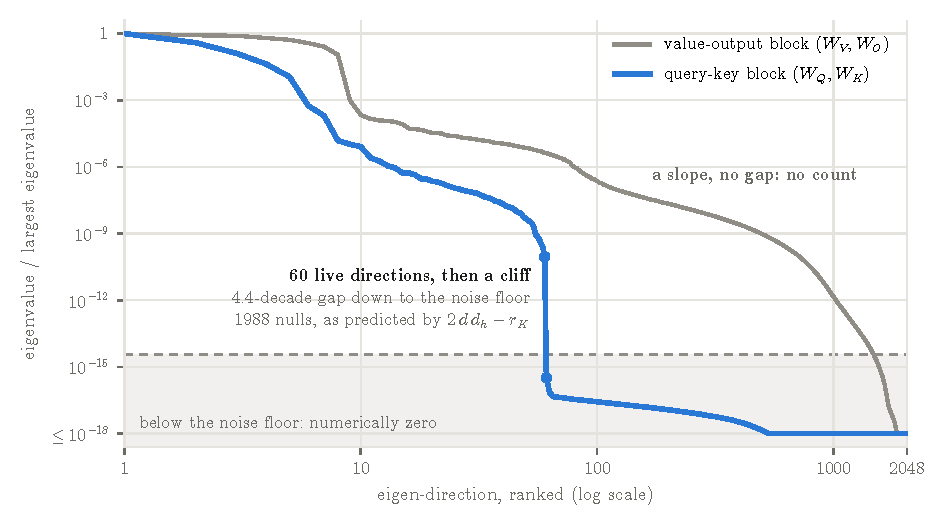
\includegraphics[width=\textwidth]{figures/head_spectra.pdf}
\caption{\textbf{Exact redundancy is a cliff; sloppiness is a slope.} Fisher eigenvalues of
the query--key and value--output blocks of head 0 (2048 parameters each), ranked and
divided by the largest. Block Fisher over all 3481 inputs, seed 0. The shaded band lies
below the noise floor ($16\,\epsilon_{\mathrm{mach}}$ relative to $\lambda_1$). Where the
redundancy is exact, the gap test counts the nulls with no rank threshold: 1988, the
number predicted from the input ranks. The value--output spectrum decays through
fourteen decades with no gap, so its nulls cannot be separated from sloppy directions
and the test gives no count. Verdicts for all heads are in \cref{tab:ident}.}
\label{fig:spectra}
\end{figure}

\begin{table}[t]
\centering\small
\caption{Gap-test verdicts ($D=3$ decades, $\mu_0=10^{-6}$, noise floor on). ``Predicted''
is the null dimension computed from data ranks (\cref{sec:stage1}). ``Arch.''\ is the part
implied by the architecture and the constant query token alone, before any rank deficiency
of the data: $2dd_h-d$ for QK, the $GL(d_h)$ gauge $d_h^2$ for OV, the positive rescaling
of a ReLU unit, and none for the sigmoid MLP.}
\label{tab:ident}
\setlength{\tabcolsep}{4.5pt}
\begin{tabular}{@{}lrlrrrrr@{}}
\toprule
block & $p_B$ & verdict & null dim. & predicted & arch. & gap (dec.) & at floor\\
\midrule
MLP, all parameters & 5301 & under-determined & 0 & -- & 0 & 0.9 & 5208\\
head 0, QK & 2048 & structural & 1988 & 1988 & 1984 & 4.41 & 1988\\
head 1, QK & 2048 & structural & 1988 & 1988 & 1984 & 4.58 & 1988\\
head 2, QK & 2048 & structural & 1988 & 1988 & 1984 & 4.87 & 1988\\
head 3, QK & 2048 & structural & 1988 & 1988 & 1984 & 3.63 & 1988\\
heads 0--3, OV & 2048 & under-determined & 0 & 320 & 256 & 2.0--2.8 & 553--601\\
four MLP units & 129 & under-determined & 0 & -- & 1 & 1.4--2.3 & 10--14\\
\bottomrule
\end{tabular}
\end{table}

\paragraph{The quotient is exact where the test says so.} Cutting the QK product of head 0
from rank 16 to rank 1 removes 1920 parameters and changes the validation loss by
$1.2\times10^{-10}$. On the MLP, zeroing the outgoing column of one of two near-duplicate
units costs $+0.027$ to $+0.029$ in validation loss, while merging them costs
$\pm4\times10^{-5}$ (\cref{cor:duplicate}).

\subsection{Round 3: Fisher-distance schemes}
\label{sec:res-berman}

Under the round-1 test, the four schemes of \citet{berman2026fdist} stop at 4--7\% of
the MLP parameters on average with the loss criterion (range 2--9\% over seeds), and at
8--12\% with the error criterion. On the transformer they stop at 6\% with the loss
criterion; with the error criterion they stop at 10\% (one-shot), 26\% (global) and 34\%
(iterative). Along the sparsity curve they beat magnitude pruning on the MLP; on the
transformer the two are close (\cref{tab:matched}). Their stop points are in the range of
the other one-shot baselines.

\subsection{Round 4: controlled comparison}
\label{sec:res-fair}

\Cref{tab:fair} is the main result. \Cref{fig:mlp,fig:tf} show the curves behind it.

\begin{table}[t]
\centering\small
\caption{Percentage of parameters ($\keff$) removed at the stop point of the common rule
(anchored paired $2\sigma$ test on $\DB$, cut at the first failure). MLP: mean over three
seeds, margin $\rho=1\%$ of the base loss. Transformer: seed 0, margin $\rho=100\%$.
One-shot entries: Berman et al.'s iterative scheme for \Wo, classical mean ablation for
\So. Test accuracy at every transformer stop point is 1.000.}
\label{tab:fair}
\begin{tabular}{@{}llccc@{}}
\toprule
model & granularity & one-shot & chosen on $\Dtr$ & chosen on $\DA$\\
\midrule
\multirow{3}{*}{MLP} & \Wo{} single parameters & 5.8 & 18.0 & 10.2\\
& \So{} structural & 14.4 & 93.8 & 95.0\\
& \WS{} & -- & 94.2 & \textbf{96.6}\\
\midrule
\multirow{3}{*}{Transformer} & \Wo{} single parameters & 14.0 & 26.7 & 27.0\\
& \So{} structural & 12.8 & 52.5 & 52.7\\
& \WS{} & -- & 65.2 & \textbf{66.3}\\
\bottomrule
\end{tabular}
\end{table}

\begin{figure}[t]
\centering
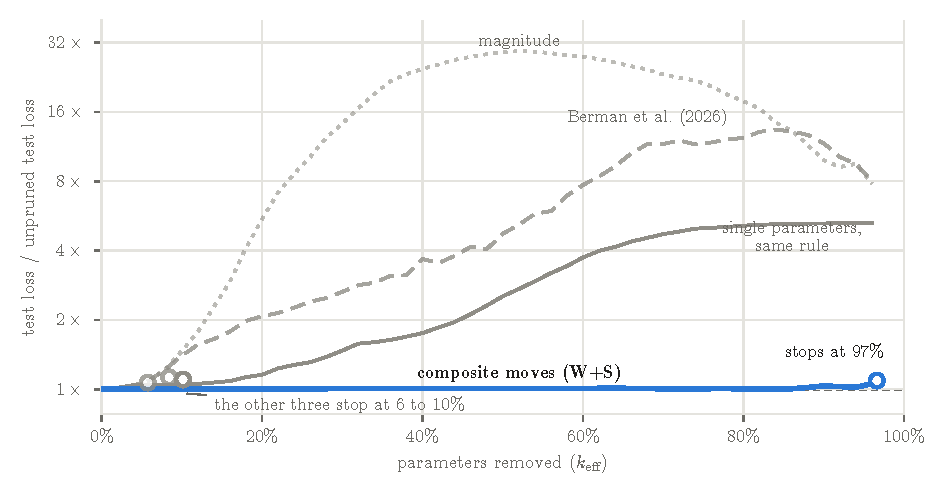
\includegraphics[width=\textwidth]{figures/mlp_loss.pdf}
\caption{\textbf{Composite moves stay within 6\% of the original loss up to 96\% removed.}
MLP test loss divided by the unpruned test loss, mean of three seeds, against the
fraction of parameters removed. Rings: where the common stop rule (margin 1\%) halts
each method, at the mean over seeds of the stop point and of the loss ratio there.
On the MLP the composite arm never leaves the unpruned loss. Every single-parameter rule
has at least doubled it before half the network is gone.}
\label{fig:mlp}
\end{figure}

\begin{figure}[t]
\centering
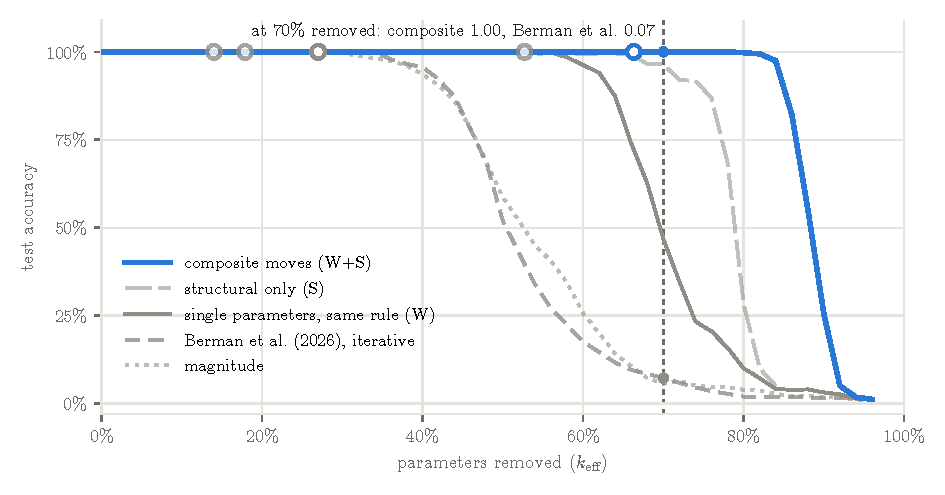
\includegraphics[width=\textwidth]{figures/tf_accuracy.pdf}
\caption{\textbf{Composite moves hold test accuracy above 99\% to 82\% removed.} Transformer
on $a+b\bmod59$, seed 0. Rings: where the stop rule (margin $=$ base loss) halts each
method. Every method stops while still at 100\% accuracy. Beyond the stops, accuracy
first falls below 99\% at 82\% removed for the composite arm, at 67\% for structural
moves alone, at 57\% for single parameters under the same rule, at 32--36\% for
magnitude and the iterative and global Fisher-distance schemes, and at 12\% for the
one-shot Fisher-distance scheme. Structural moves alone run out near 85\%, because the embeddings and the
unembedding (14\% of the parameters) have no structural moves.}
\label{fig:tf}
\end{figure}

\paragraph{Finding 1: held-out data in the loop is not where the advantage comes from.}
Choosing each move on training data gives essentially the same result as choosing it on
$\DA$. On the MLP: \WS{} 94\% vs 97\%, \So{} 94\% vs 95\%. On the transformer: \WS{} 65\%
vs 66\%, \So{} 52\% vs 53\%. For single parameters, choosing on training data is even
slightly better on the MLP (18\% vs 10\%), presumably because $\Dtr$ is six times larger
than $\DA$ and ranks small differences better.

\paragraph{Finding 2: composite moves are where it comes from.} The proposer, the
tie-break and the stop rule are the same in every arm. Even so, structural arms remove
94--97\% of the MLP, single-parameter greedy arms 10--21\%, and the one-shot Fisher
distances 6--9\% (\cref{tab:margins}). At matched sparsity (\cref{tab:matched}), the
structural arms keep the base test loss up to 90\% removed (ratio $\le1.03$). The best
single-parameter arm has $2.4\times$ the base loss at 50\% removed. At their stop points the structural arms have test loss 1--15\% above the original, with
unchanged test accuracy. This is the same range as the single-parameter arms at their much
earlier stops (7--22\%). On the transformer, test accuracy at 70\% removed is $1.00$ for \WS, $0.47$--$0.50$ for greedy single
parameters with the Fisher-distance proposer ($0.23$ with magnitude), $0.07$ for Berman's iterative scheme and $0.06$ for magnitude. Here the
combination matters: \WS{} beats \So{} alone. The embeddings and the unembedding (14\% of
the parameters) have no structural moves, and \So{} is less accurate at 70\% ($0.85$--$0.96$).

\paragraph{Finding 3: greedy evaluation helps single parameters, but only moderately.}
Evaluating each single-parameter move on data lifts the MLP stop from 6\% (one-shot) to
10--21\%. On the transformer it lifts accuracy at 50\% removed from $0.52$ to $0.999$.
One-shot structural pruning, i.e.\ classical mean ablation, stays poor: 14\% on the
MLP and 13\% on the transformer. Composite moves pay off only when each one is
evaluated.

\paragraph{Finding 4: the pure $2\sigma$ rule needs a practical margin.} With $\rho=0$,
the MLP stop points of \WS{} on $\DA$ are 95\%, 10\% and 83\% across the three seeds.
A step with a tiny but systematic loss change ends the path, even though later steps
pass again (\cref{sec:decide}). Any margin $\rho\ge0.5\%$ removes the bimodality
(\cref{tab:margins}). On the transformer, $\rho=0$ and $\rho=1\%$ differ by at most two points. At every
margin the structural arms stay far above the single-parameter arms, which stay above
the one-shot schemes. The finer order can change: at $\rho=0$, \So{} beats \WS.

\begin{table}[t]
\centering\small
\caption{Stop point (\% of $\keff$ removed) as a function of the margin $\rho$ (fraction of
the base validation loss). MLP: mean over three seeds.}
\label{tab:margins}
\setlength{\tabcolsep}{4.2pt}
\begin{tabular}{@{}lcccc@{\hspace{1.0em}}ccccc@{}}
\toprule
& \multicolumn{4}{c}{MLP, $\rho=$} & \multicolumn{5}{c}{Transformer, $\rho=$}\\
\cmidrule(r{1.2em}){2-5}\cmidrule{6-10}
method & 0 & 0.5\% & 1\% & 2\% & 0 & 1\% & 10\% & 100\% & 1000\%\\
\midrule
\WS{} on $\DA$ & 62.6 & 91.5 & 96.6 & 96.9 & 43.7 & 44.3 & 48.5 & 66.3 & 77.2\\
\WS{} on $\Dtr$ & 63.9 & 93.7 & 94.2 & 96.3 & 47.9 & 48.2 & 51.5 & 65.2 & 78.1\\
\WS{} on $\DA$, OBD proposer & 66.0 & 94.9 & 94.9 & 94.9 & 32.8 & 33.2 & 50.0 & 62.1 & 70.1\\
\So{} on $\DA$ & 65.7 & 94.9 & 95.0 & 95.0 & 44.2 & 44.4 & 47.5 & 52.7 & 53.1\\
\So{} on $\Dtr$ & 63.6 & 93.2 & 93.8 & 96.1 & 43.3 & 43.9 & 47.8 & 52.5 & 52.7\\
\Wo{} on $\DA$ & 10.2 & 10.2 & 10.2 & 18.8 & 7.9 & 8.7 & 16.7 & 27.0 & 40.5\\
\Wo{} on $\Dtr$ & 15.7 & 17.0 & 18.0 & 21.8 & 8.0 & 9.0 & 14.2 & 26.7 & 40.3\\
\Wo{} on $\DA$, magnitude proposer & 18.9 & 20.4 & 21.0 & 21.4 & 8.6 & 9.2 & 15.0 & 26.1 & 37.7\\
\midrule
Berman et al., iterative & 5.1 & 5.8 & 5.8 & 5.8 & 8.0 & 8.0 & 10.0 & 14.0 & 28.0\\
Berman et al., exact & 5.1 & 5.8 & 5.8 & 5.8 & -- & -- & -- & -- & --\\
Berman et al., global & 7.7 & 7.7 & 9.3 & 9.3 & 6.0 & 6.0 & 8.0 & 10.0 & 18.0\\
Berman et al., one-shot & 5.1 & 5.8 & 5.8 & 5.8 & 6.0 & 6.0 & 6.0 & 8.0 & 10.0\\
magnitude & 8.4 & 8.4 & 8.4 & 8.4 & 4.0 & 6.0 & 9.9 & 17.9 & 23.8\\
mean ablation & 11.8 & 13.4 & 14.4 & 16.1 & 0.0 & 0.9 & 3.8 & 12.8 & 21.8\\
\bottomrule
\end{tabular}
\end{table}

\begin{table}[t]
\centering\small
\caption{Test metric at matched sparsity (linear interpolation along each path; MLP: mean
of three seeds). ``--'': the method's path does not reach that sparsity.}
\label{tab:matched}
\setlength{\tabcolsep}{4.2pt}
\begin{tabular}{@{}lccccc@{\hspace{1.0em}}ccccc@{}}
\toprule
& \multicolumn{5}{c}{MLP: test loss / base, at removed} & \multicolumn{5}{c}{Transformer: test accuracy, at removed}\\
\cmidrule(r{1.2em}){2-6}\cmidrule{7-11}
method & 10\% & 30\% & 50\% & 70\% & 90\% & 10\% & 30\% & 50\% & 70\% & 90\%\\
\midrule
\WS{} on $\DA$ & 1.00 & 1.01 & 1.01 & 1.00 & 1.03 & 1.00 & 1.00 & 1.00 & 1.00 & 0.26\\
\WS{} on $\Dtr$ & 1.00 & 1.00 & 1.00 & 1.00 & 1.02 & 1.00 & 1.00 & 1.00 & 1.00 & 0.18\\
\So{} on $\DA$ & 1.00 & 1.00 & 1.00 & 1.00 & 1.02 & 1.00 & 1.00 & 1.00 & 0.96 & --\\
\So{} on $\Dtr$ & 1.00 & 1.00 & 1.00 & 1.00 & 1.02 & 1.00 & 1.00 & 1.00 & 0.85 & --\\
\Wo{} on $\DA$ & 1.05 & 1.47 & 2.53 & 4.72 & 5.24 & 1.00 & 1.00 & 1.00 & 0.47 & 0.03\\
\Wo{} on $\Dtr$ & 1.04 & 1.28 & 2.40 & 4.35 & 5.15 & 1.00 & 1.00 & 1.00 & 0.50 & 0.03\\
\Wo{} on $\DA$, magnitude & 1.07 & 1.41 & 2.42 & 4.58 & 5.22 & 1.00 & 1.00 & 0.98 & 0.23 & 0.02\\
\midrule
Berman et al., iterative & 1.40 & 2.65 & 4.73 & 11.6 & 11.7 & 1.00 & 1.00 & 0.52 & 0.07 & 0.02\\
Berman et al., global & 1.17 & 3.09 & 8.50 & 19.8 & 12.7 & 1.00 & 0.99 & 0.21 & 0.06 & 0.02\\
Berman et al., one-shot & 1.55 & 13.3 & 22.1 & 13.2 & 8.18 & 1.00 & 0.25 & 0.28 & 0.12 & 0.02\\
magnitude & 1.46 & 14.2 & 29.1 & 23.2 & 9.86 & 1.00 & 1.00 & 0.59 & 0.06 & 0.02\\
mean ablation & 1.03 & 1.34 & 3.09 & 4.99 & 5.24 & 1.00 & 0.99 & 0.29 & 0.03 & --\\
random & 1.33 & 2.01 & 2.29 & 4.17 & 5.13 & 0.59 & 0.02 & 0.01 & 0.01 & 0.01\\
\bottomrule
\end{tabular}
\end{table}

\paragraph{Which moves do the work.} \Cref{tab:composition} breaks the removed parameters
down by move kind, up to the stop point. On the MLP, merges of near-duplicate units
account for 90--95\% of all parameters in every seed. Mean replacement, saturation and
a few weight chunks account for the rest. Across the 24 MLP paths of round 4, a
Heaviside move is accepted before the stop point exactly once. On the
transformer the work is spread out. Merges remove 25--29\%, QK and OV rank cuts 21--22\%,
and weight chunks 10\% in \WS. The QK cuts are the striking part. In the \So{} arm the
loop cuts the QK product of every head from rank 16 to rank 1 (15 cuts per head). In
\WS{} it does so in three heads and leaves the fourth at rank 2. This is the exact
quotient that Stage 1 predicts (\cref{sec:stage1}), found by 59--60 held-out decisions.
A Stage-1 implementation would make those decisions free. The OV products are cut by
9--10 ranks per head, to rank 6 or 7. These cuts are sloppy, not exact, and were
decided by data.

\begin{table}[t]
\centering\small
\caption{Parameters removed by each move kind up to the stop point, as a percentage of the
original $p$ (number of accepted moves in brackets). MLP: seed 123, margin 1\%;
transformer: margin $=$ base loss.}
\label{tab:composition}
\begin{tabular}{@{}lcccc@{}}
\toprule
& \multicolumn{2}{c}{MLP} & \multicolumn{2}{c}{Transformer}\\
\cmidrule(r){2-3}\cmidrule(l){4-5}
move kind & \WS{} on $\DA$ & \So{} on $\DA$ & \WS{} on $\DA$ & \So{} on $\DA$\\
\midrule
\code{unit\_merge} & 93.2 (91) & 94.9 (89) & 29.4 (137) & 25.2 (112)\\
\code{unit\_mean} & 0.4 (4) & 1.9 (9) & 4.3 (27) & 4.7 (21)\\
\code{unit\_sat} & 0.5 (3) & 0.2 (3) & 1.3 (9) & 0.9 (4)\\
\code{qk\_rank} & -- & -- & 13.2 (59) & 13.4 (60)\\
\code{ov\_rank} & -- & -- & 8.1 (37) & 8.5 (38)\\
\code{zero} & 3.6 (13) & -- & 10.0 (89) & --\\
\midrule
total removed (with cascades) & 97.7 & 97.0 & 66.3 & 52.7\\
\bottomrule
\end{tabular}
\end{table}

% =============================================================================
\section{Discussion}
\label{sec:discussion}

\subsection{What the evidence supports}

On both toy models, a single decision rule over boundary moves removes far more
parameters than single-parameter pruning before the same held-out test fails. The
controlled design attributes the gain to the composite moves themselves. Using
held-out data to choose the moves makes little difference, and evaluating
single-parameter moves greedily helps them only moderately. One-shot structural pruning
does not reproduce the gain. The gap test does what it is meant to do. It returns an
exact count where the redundancy is exact (QK) and that count matches an independent
prediction. Where the redundancy is buried in a sloppy slope (OV, the MLP) it refuses to
count. \Cref{prop:singular} explains why a coordinate Fisher length cannot see the
cheapest reductions of a singular model: these run along null directions, and the
coordinate path does not. The duplicate-unit and QK examples show the effect in
numbers.

\subsection{What it does not show yet}
\label{sec:threats}

\begin{itemize}
\item \textbf{Scale and realism.} Two toy tasks, three MLP seeds and one transformer
seed. The moons MLP is heavily over-parametrised for its task, and many near-duplicate
units are expected there. The transformer task is algorithmic and has zero Bayes error.
\item \textbf{Compensation.} Structural moves carry closed-form compensation (folds,
merges, weighted SVD), and single-parameter moves carry none. Part of what we call the
``composite'' advantage may be the ``compensated'' advantage, which OBS-type methods
also provide at the single-parameter level
\citep{hassibi1993obs,frantar2023sparsegpt}.
\item \textbf{Baselines.} The baselines are post-training and without compensation or
fine-tuning. The strongest modern pruners (SparseGPT, per-row Wanda, FLAP,
\citealp{kwon2022fast}) are not yet included. Neither is the common protocol of
fine-tuning after pruning.
\item \textbf{Complexity count.} $\keff$ counts parameters, not FLOPs or latency.
Merges and rank cuts shrink real widths, while scattered zeros do not. Continuous gauges
are not subtracted.
\item \textbf{Statistics.} The margin $\delta$ is chosen by hand. Along a path, the
stop test is applied many times without multiplicity control. The decision is a
tolerance rule, not a calibrated test. The resolution limit \eqref{eq:resolution}
caps what any paired test on $n$ samples can see.
\item \textbf{Moves that did little.} Saturation and Heaviside moves, the moves that are
new as pruning moves, contributed almost nothing on these tasks (\cref{tab:composition}).
\end{itemize}

% =============================================================================
\section{Outlook: what is needed for a credible paper}
\label{sec:outlook}

\Cref{tab:outlook} lists the open items, ordered by how much each would change the
credibility of the claims.

\begin{table}[htbp]
\centering\footnotesize
\caption{Open items. Priority A: the headline claims are not credible without it.
B: needed for a complete paper. C: strengthens or extends.}
\label{tab:outlook}
\renewcommand{\arraystretch}{1.25}
\begin{tabularx}{\textwidth}{@{}p{0.4cm}p{3.6cm}Xp{1.0cm}@{}}
\toprule
& \textbf{Item} & \textbf{What to do, and what it would show} & \textbf{Prio.}\\
\midrule
1 & Real task, deeper model & A multi-layer transformer on a real task (character-level or TinyStories language model) with LayerNorm. At least five seeds, with confidence intervals over seeds and bootstrap intervals over test samples. Shows that the gain is not an artefact of over-parametrised toys. & A\\
2 & Compensation ablation & Structural moves without their fold or merge, and single-parameter moves with OBS/SparseGPT-style least-squares compensation. Separates ``composite'' from ``compensated''. & A\\
3 & Stronger baselines & SparseGPT, per-row Wanda, FLAP, \citet{kwon2022fast}, SliceGPT and LLM-Pruner, each with and without a short fine-tuning budget shared by all methods. Every method under the same $\DB$ stop rule. & A\\
4 & Stage 1 as its own step & Implement \cref{alg:stage1}: quotient moves for structural verdicts with a numerical identity check. Measure the held-out decisions it saves (60 on the toy transformer). Extend the null predictions of \cref{sec:stage1} to models in which the query input is not constant. & B\\
5 & Efficiency metrics & FLOPs, latency and memory next to $\keff$. Report structured and unstructured sparsity separately. Choose the chunk size so that the $\keff$ tie-break does not favour large chunks. & B\\
6 & Statistical protocol & A principled margin, e.g.\ a task-level tolerance analogous to the relative tolerance $\beta$ of the SR gate. A sensitivity analysis over $\rho$ and $n_\sigma$. Treat the stop rule as an equivalence test. Size $\DB$ by a power analysis using \eqref{eq:resolution}. Guard against reuse of $\DB$ across methods and settings \citep{dwork2015reusable}. & B\\
7 & Hyperparameter sensitivity & Sweeps over candidate budgets, refresh interval and screen size, as in the sensitivity study of the SR paper. & B\\
8 & Softmax infinities & Single-token masking (one logit $\to-\infty$) and input-dependent hard-max ($s\to\infty$). Test them on sink or hard heads of a deeper model. & B\\
9 & Where saturation should matter & Sigmoid-gated architectures (GLU, LSTM), networks driven into saturation, inputs with thresholds. If the saturation and step moves stay inactive, drop them from the claims. & C\\
10 & Singularity-aware complexity & Estimate the local learning coefficient \citep{lau2025llc} before and after pruning, as an analysis of $\keff$ (not as a tie-break). Do pruned networks with equal $\keff$ differ in learning coefficient? & C\\
11 & Theory & State the stratification of the compactified parameter space that the moves visit. Give conditions for uniform convergence of the limits (e.g.\ sigmoid saturation on compact inputs). Prove that quotient moves are exact for the predicted nulls. Bound the cumulative loss change implied by the anchored rule. & C\\
12 & Interpretation & Read the pruned transformer: QK at rank 1 and OV at rank 6--7 per head. Does the remaining circuit expose the known algorithm for modular addition \citep{nanda2023progress}? & C\\
13 & Fairness details & Let the single-parameter arm prune biases, as Berman et al.'s protocol does. Make the $\keff$ tie-break and the chosen margin the package defaults. & C\\
\bottomrule
\end{tabularx}
\end{table}

The most informative next experiment is item 1 together with item 2: a deeper
transformer on a real task, with and without compensation in the structural moves.
If the composite advantage survives both, the controlled design of \cref{sec:fair} can
be rerun at that scale against the baselines of item 3.

\FloatBarrier

% =============================================================================
\appendix

\section{Weighted low-rank truncation}
\label{app:wsvd}

\paragraph{Objective.} Let $x_q,x_k\in\R^{d}$ be independent with second moments
$C_q=\E[x_qx_q^{\top}]$ and $C_k=\E[x_kx_k^{\top}]$, and let $\Delta\in\R^{d\times d}$.
Then
\[
\E\big[(x_q^{\top}\Delta x_k)^2\big]
=\E\big[x_q^{\top}\Delta\,x_kx_k^{\top}\,\Delta^{\top}x_q\big]
=\E\big[x_q^{\top}\Delta C_k\Delta^{\top}x_q\big]
=\operatorname{tr}\big(\Delta C_k\Delta^{\top}C_q\big)
=\big\|C_q^{1/2}\Delta\,C_k^{1/2}\big\|_F^{2}.
\]
In the transformer the query and key inputs of one sequence are not independent, so
this identity motivates \eqref{eq:wsvd} rather than equating it with the expected
squared logit change. For the OV product, with $y=\sum_sA_{Ts}x_s$,
$\E\|y^{\top}(N-N')\|^2=\operatorname{tr}\big((N-N')^{\top}C_y(N-N')\big)=
\|C_y^{1/2}(N-N')\|_F^2$ holds without any independence assumption.

\paragraph{Minimiser.} Suppose $C_q,C_k\succ0$, which the eigenvalue floor guarantees.
The map $M'\mapsto N'=C_q^{1/2}M'C_k^{1/2}$ is a bijection that preserves rank, and the
objective is $\|C_q^{1/2}MC_k^{1/2}-N'\|_F$. By the Eckart--Young theorem the minimiser
over $\rank N'\le r-1$ is the truncated SVD $N'=U_{r-1}\Sigma_{r-1}V_{r-1}^{\top}$ of
$C_q^{1/2}MC_k^{1/2}$. Hence $M'=C_q^{-1/2}N'C_k^{-1/2}=W_Q'W_K'^{\top}$, with the
factors of \cref{sec:moves-tf}. The floor replaces each $C$ by
$V\max(\Lambda,\epsilon\lambda_{\max})V^{\top}$ with $\epsilon=10^{-8}$. Directions with
no data weight then contribute almost nothing to the objective, and $C^{-1/2}$ does not
amplify them. This also avoids the negative eigenvalues that rounding produces in
nearly singular covariances.

\section{Reproducibility}
\label{app:repro}
\sloppy

Everything is in \code{Pruning\_framework/NNpruning/}. The package \code{nnprune/}
contains:
\begin{itemize}
\item \code{core.py}: states, moves, the decision rule, the greedy path and the baselines;
\item \code{mlp.py} and \code{transformer.py}: the two adapters (moves, folds, cascades,
data, training);
\item \code{spectrum.py}: the gap classifier with noise floor, the block Fisher and the
predicted nulls;
\item \code{fdist\_baseline.py} and \code{third\_party/}: Berman et al.'s schemes, with
their Fisher code vendored under its Apache-2.0 licence;
\item \code{experiments.py}: drivers with CSV caching.
\end{itemize}
Any round is rerun from the command line with
\begin{center}\code{python run\_experiments.py} \textit{round},\end{center}
where \textit{round} is one of \code{mlp}, \code{mlp-spectrum}, \code{transformer},
\code{fdist-mlp}, \code{fdist-transformer}, \code{fair-mlp} and \code{fair-transformer}. The notebooks
\code{NNpruning.ipynb} (rounds 1--3) and \code{fair\_comparison.ipynb} (round 4) load the
cached results by default. The script \code{make\_figures.py} in \code{paper/} regenerates
\cref{fig:mlp,fig:tf,fig:spectra} and prints every matched-sparsity number in
\cref{tab:matched}. With the defaults, every flag added for the controlled design
(\code{select\_split}, \code{stop\_split}, \code{stop\_mode},
\code{select\_admissibility}, \code{post\_stop\_steps}, \code{max\_frac},
\code{weight\_score}) reproduces round 1 bit for bit. On a laptop CPU, round 1 takes about 10 minutes per MLP seed and about one hour for the
transformer (all variants and baselines). Round 4 takes about 40 minutes for the MLP
(three seeds) and 1.5 hours for the transformer. The test suite has 15 core tests and 5
faithfulness tests against Berman et al.'s own pruner classes; the latter need their
repository and \code{nngeometry}.

\bibliographystyle{plainnat}
\bibliography{refs}

\end{document}
